\documentclass[nolayout]{article}

\usepackage[utf8]{inputenc}
\usepackage[english]{babel}
\usepackage{amsmath,amsthm}
\usepackage{geometry}
\usepackage{tikz}
\usetikzlibrary{fit,positioning}
\usepackage[textwidth=4cm,textsize=footnotesize]{todonotes}
\usepackage{fancyhdr}
\pagestyle{fancy}
\usepackage{amssymb,color,bbm,xargs}
\usepackage{graphicx}
\usepackage[active]{srcltx}
\usepackage{ifthen}
\usepackage{enumerate}
\usepackage{dsfont}
\usepackage{subcaption}

\newtheorem{lemma}{Lemma}
\newtheorem{proposition}{Proposition}
\newtheorem{theorem}{Theorem}
\newtheorem{corollary}{Corollary}

\definecolor{lavander}{cmyk}{0,0.48,0,0}
\definecolor{violet}{cmyk}{0.79,0.88,0,0}
\definecolor{burntorange}{cmyk}{0,0.52,1,0}
\definecolor{burntgreen}{cmyk}{0.62,0.44,0.47,0}
\definecolor{burntblue}{cmyk}{0.86,0.30,0.18,0}
\definecolor{palegreen}{cmyk}{0.86,0.30,0.96,0}


\def\sup{\mathrm{sup}}
\def\param{\theta}
\def\paramset{\Theta}
\def\1{\mathds{1}}
\def\rset{\mathbb{R}}
\def\rmd{\mathrm{d}}
\def\eqsp{\,}
\def\Pstar{\mathbb{P}_{\pi_{\star}}}
\def\bayes{\pi_{\star}}
\def\kernel{\mathsf{M}}
\newcommand{\limit}[1]{\underset{#1\to \infty}{\longrightarrow}}
\newcommand{\E}{\mathbb{E}}
\newcommand{\kullback}{\mathsf{L}}
\newcommand{\link}{\leftrightarrow}


\newcommand{\pa}[1]{\left(#1\right)}
\newcommand{\cro}[1]{\left[#1\right]}
\newcommand{\set}[1]{\left\{#1\right\}}
\newcommand{\PE}[1]{\left\lfloor#1\right\rfloor}

\newcommand{\loss}[1]{\ell\pa{#1}}
\newcommand{\Lo}[2]{\ell^{#1}\pa{#2}}

\newcommand{\bN}{\mathbb{N}}
\newcommand{\bP}{\mathbb{P}}
\newcommand{\bR}{\mathbb{R}}
\newcommand{\bZ}{\mathbb{Z}}

\newcommand{\cA}{\mathcal{A}}
\newcommand{\cD}{\mathcal{D}}
\newcommand{\cE}{\mathcal{E}}
\newcommand{\cO}{\mathcal{O}}
\newcommand{\cS}{\mathcal{S}}
\newcommand{\cV}{\mathcal{V}}
\newcommand{\cX}{\mathcal{X}}

\newcommand{\ordermax}[2]{{\mathsf{q}}^{#1}_{#2}}
\newcommand{\remainder}[2]{{\mathsf{r}}^{#1}_{#2}}

\newcommand{\condlik}{k}
\newcommand{\card}{\mathrm{card}}

\newcommand{\MLE}{\widehat{\pi}}

\newcounter{hypH}
\newenvironment{hypH}{\refstepcounter{hypH}\begin{itemize}
\item[{\bf H\arabic{hypH}}]}{\end{itemize}}
\begin{document}

\title{Early learning in Bradley-Terry tournaments}
\date{}

\author{}

\lhead{}
\rhead{MLE for the Bradley-Terry tournaments in random environment}

\maketitle

\begin{abstract}

\end{abstract}

\section{Introduction}
The Bradley-Terry model introduced in \cite{bradley:terry:1952,zemerlo:1929} is a popular approach to describe the outcomes of paired comparisons in a contest involving $N$ players, written $[N]=\{1,\ldots,N\}$. For all $1\le i \ne j\le N$, the odds that $i$ beats $j$ is $v_i/(v_i+v_j)$ where $(v_i)_{1\le i\le N}$ are positive numbers representing the 'abilities' or 'overall skills' of  the players. This model has been generalized in many directions and applied to a wide range of experimental data, see for instance \cite{stigler:1994} to quantify the intellectual influence between statistical journals...
\cite{hastie:tibshirani:1998}
\cite{hunter:2004}
\section{Bradley-Terry tournament (BTT) in random environment}
Consider a tournament involving an even number $N$ of players called $[N]=\{1,\ldots,N\}$. 
During the tournament, players face each other at most once and, when $i$ faces $j$ for $1\le i \neq j\le N$, write $X_{i,j}=1$ if $i$ beats $j$ and $X_{i,j}=0$ if $j$ beats $i$, in particular $X_{i,j}=1-X_{j,i}$. With each player $1\le i\le N$ is associated an 'ability parameter' $v_i>0$ where $v=(v_i)_{i\in[N]}$ are assumed to be independent and identically distributed with unknown probability density function $\bayes$ with respect to the Lebesgue measure. Conditionally on $v=(v_i)_{i\in[N]}$, the random variables $(X_{i,j})_{1\le i<j\le N}$ are independent and such that:
\[
\bP(X_{i,j}=1|v) = \bP(X_{i,j}=1|v_i,v_j)=\frac{v_i}{v_i+v_j}\enspace.
\]
To ease notation, for every vector $a\in \bR^p$ and every subset $B\subset [p]=\{1,\ldots,p\}$, we denote by $a_{B}=\{a_i,\;i\in B\}$. Define, for all $x\in \{0,1\}$ and all $(v_1,v_2)\in(\bR_+^*)^2$, 
\begin{equation}
\label{eq:def:condlik}
\condlik(x,v_{[2]})=\frac{v_1^xv_2^{1-x}}{v_1+v_2}\enspace,
\end{equation}
so that $\bP(X_{i,j}=x|v_{\{i,j\}})=k(x,v_{\{i,j\}})$. 
%In our model, $v=(v_i)_{i\in [N]}$ is a vector in $\bR^N$ with i.i.d. entries with common unknown distribution $\bayes$ that is set once and for all before the tournament begins. 


\subsection{Round-robin days in BTT and early learning task}
In this paper, it is not assumed that all the pairs meet once, each contestant meets others in turn according to  the round-robin scheduling that gives at each time $t\in[N]$ the pairs that face each others. At time $t=1$, this algorithm pairs the players off according to Figure~\ref{fig:robin:day1}. Each player faces the one in front of him, that is $2i-1$ faces $2i$, for all $i\in[N/2]$. At time $t=2$, a player is fixed and all the others are rotated clockwise as described in Figure~\ref{fig:robin:move}. Player $1$ does not move, $2$ takes the place of $3$, each odd integer $2i-1<N-1$ takes the place of $2i+1$, $N-1$ takes the place of $N$ and each even integer $2i>2$ takes the place of $2(i-1)$. Once they moved, each player faces the opponent in front of him. At time $t\ge 2$, each player moves once according to the round-robin algorithm and plays the opponent in front of him as displayed in Figure~\ref{fig:robin:day2}. Each time $t\in\bN$ is called a day of the tournament. It is well known that, at day $N$, all players have faced each other once. 

In this paper, it is assumed that the results of $n$ games are available and the distribution $\bayes$ is estimated using this data set. The time $n$ is assumed to be much smaller than $N$ this problem is therefore referred to as the ``early learning task". The set of couples $(i,j)\in[N]^2$, with $i<j$ such that $i$ has played $j$ before time $n$ is denoted by $\cA_{n,N}$, in other words, the data set is $\cD_{n,N}=\{(X_{i,j})_{(i,j)\in A_{n,N}}\}$.

\begin{figure}[h!]
\begin{subfigure}{\textwidth}
  \centering
  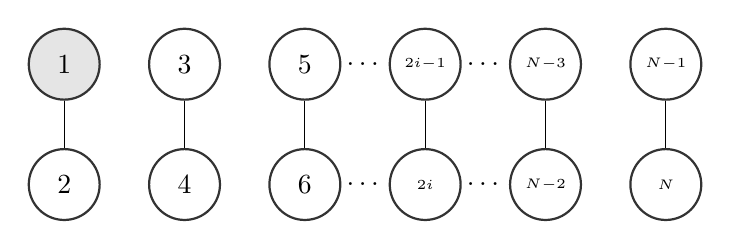
\begin{tikzpicture}
\tikzstyle{main}=[circle, minimum size = 9mm, thick, draw =black!80, node distance = 6mm]
\tikzstyle{connect}=[-latex, thick]
\tikzstyle{box}=[rectangle, draw=black!100]
\node[main, fill = black!10] (v1){$1$ };
\node[main] (v3) [right=of v1] {$3$ };
\node[main] (v5) [right=of v3] {$5$ };
\node[main] (v7) [right=of v5] {${\scriptscriptstyle 2i-1}$};
\node[main] (v9) [right=of v7] {${\scriptscriptstyle N-3}$};
\node[main] (v11) [right=of v9] {${\scriptscriptstyle N-1}$};
\node[main] (v2) [below=of v1] {$2$};
\node[main] (v4) [below=of v3] {$4$};
\node[main] (v6) [below=of v5] {$6$};
\node[main] (v8) [below=of v7] {${\scriptscriptstyle 2i}$};
\node[main] (v10) [below=of v9] {${\scriptscriptstyle N-2}$};
\node[main] (v12) [below=of v11] {${\scriptscriptstyle N}$};
\draw (v1) -- (v2);
\draw (v3) -- (v4);
\draw (v5) -- (v6);
\draw (v7) -- (v8);
\draw (v9) -- (v10);  
\draw (v11) -- (v12);     
\path (v5) -- node[auto=false]{\ldots}  (v7); 
\path (v7) -- node[auto=false]{\ldots}  (v9); 
\path (v6) -- node[auto=false]{\ldots}  (v8); 
\path (v8) -- node[auto=false]{\ldots}  (v10);    
\end{tikzpicture}
\caption{Round-robin, day $1$.}
\label{fig:robin:day1}
\end{subfigure}

\vspace{.5cm}

\begin{subfigure}{\textwidth}
  \centering
  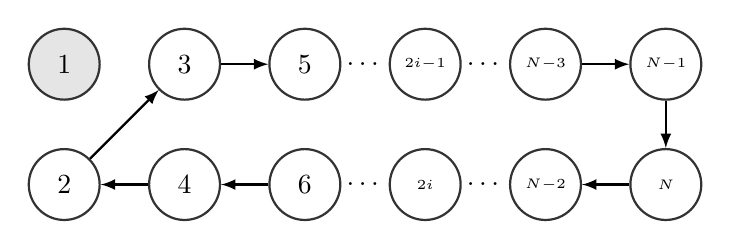
\begin{tikzpicture}
\tikzstyle{main}=[circle, minimum size = 9mm, thick, draw =black!80, node distance = 6mm]
\tikzstyle{connect}=[-latex, thick]
\tikzstyle{box}=[rectangle, draw=black!100]
\node[main, fill = black!10] (v1){$1$ };
\node[main] (v3) [right=of v1] {$3$ };
\node[main] (v5) [right=of v3] {$5$ };
\node[main] (v7) [right=of v5] {${\scriptscriptstyle 2i-1}$};
\node[main] (v9) [right=of v7] {${\scriptscriptstyle N-3}$};
\node[main] (v11) [right=of v9] {${\scriptscriptstyle N-1}$};
\node[main] (v2) [below=of v1] {$2$};
\node[main] (v4) [below=of v3] {$4$};
\node[main] (v6) [below=of v5] {$6$};
\node[main] (v8) [below=of v7] {${\scriptscriptstyle 2i}$};
\node[main] (v10) [below=of v9] {${\scriptscriptstyle N-2}$};
\node[main] (v12) [below=of v11] {${\scriptscriptstyle N}$};
\path (v2) edge [connect] (v3);   
\path (v4) edge [connect] (v2);  
\path (v3) edge [connect] (v5);  
\path (v6) edge [connect] (v4); 
\path (v9) edge [connect] (v11); 
\path (v11) edge [connect] (v12);   
\path (v12) edge [connect] (v10);   
\path (v5) -- node[auto=false]{\ldots}  (v7); 
\path (v7) -- node[auto=false]{\ldots}  (v9); 
\path (v6) -- node[auto=false]{\ldots}  (v8); 
\path (v8) -- node[auto=false]{\ldots}  (v10);    
\end{tikzpicture}
\caption{Round-robin, first move.}
\label{fig:robin:move}
\end{subfigure}

\vspace{.5cm}

\begin{subfigure}{\textwidth}
\centering
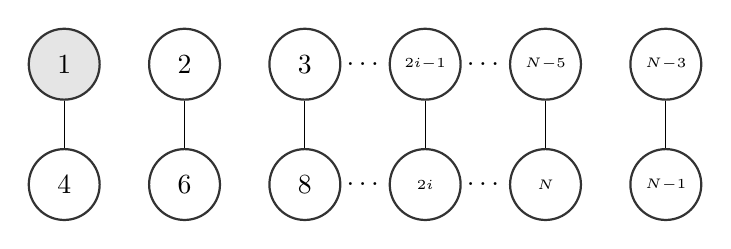
\begin{tikzpicture}
\tikzstyle{main}=[circle, minimum size = 9mm, thick, draw =black!80, node distance = 6mm]
\tikzstyle{connect}=[-latex, thick]
\tikzstyle{box}=[rectangle, draw=black!100]
\node[main, fill = black!10] (v1){$1$ };
\node[main] (v3) [right=of v1] {$2$ };
\node[main] (v5) [right=of v3] {$3$ };
\node[main] (v7) [right=of v5] {${\scriptscriptstyle 2i-1}$};
\node[main] (v9) [right=of v7] {${\scriptscriptstyle N-5}$};
\node[main] (v11) [right=of v9] {${\scriptscriptstyle N-3}$};
\node[main] (v2) [below=of v1] {$4$};
\node[main] (v4) [below=of v3] {$6$};
\node[main] (v6) [below=of v5] {$8$};
\node[main] (v8) [below=of v7] {${\scriptscriptstyle 2i}$};
\node[main] (v10) [below=of v9] {${\scriptscriptstyle N}$};
\node[main] (v12) [below=of v11] {${\scriptscriptstyle N-1}$};
\draw (v1) -- (v2);
\draw (v3) -- (v4);
\draw (v5) -- (v6);
\draw (v7) -- (v8);
\draw (v9) -- (v10);  
\draw (v11) -- (v12);     
\path (v5) -- node[auto=false]{\ldots}  (v7); 
\path (v7) -- node[auto=false]{\ldots}  (v9); 
\path (v6) -- node[auto=false]{\ldots}  (v8); 
\path (v8) -- node[auto=false]{\ldots}  (v10);    
\end{tikzpicture}
\caption{Round-robin, day $2$.}
\label{fig:robin:day2}
\end{subfigure}
\caption{First two days using the round-robin algorithm.}
\label{fig:fig}
\end{figure}

\subsection{Estimation of the environment distribution}
Our estimation strategy is quite standard. Let $\Pi$ denote a set of densities $\pi$ on $\bR_+^*$. For technical reasons, every $\pi\in\Pi$ assumed to be supported in $[\epsilon,1]$ for some $\epsilon>0$. The log-likelihood of the observations is defined, for all $\pi\in\Pi$, by:
\[
\Lo{\cD_{n,N}}{\pi}:=-\log\cro{p^{\pi}(X_{A_{n,N}})},\quad \text{where}\quad p^{\pi}(X_{A_{n,N}})=\int  \pa{\prod_{(i,j)\in A_{n,N}}k(X_{i,j},v_{\{i,j\}})}\pi^{\otimes N}(dv)\enspace.
\]
Our estimator is then any maximum likelihood estimator (MLE):
\[
\MLE\in \arg\min_{\pi\in\Pi}\{\Lo{\cD_{n,N}}{\pi}\}\enspace.
\]
We shall often forget the dependence of the log-likelihood in the data set $\cD_{n,N}$ and write $\loss{\pi}=\Lo{\cD_{n,N}}{\pi}$.

%\begin{enumerate}
%\item On pourrait supposer que toutes les lois sont a support dans un meme compact plutot que dans $[\epsilon,1]$, c'est equivalent par invariance par changement d'echelle.
%\end{enumerate}

\section{Loss of memory properties in the early learning problem}

In this section, we assume that $N\to\infty$ and $n\ll N$.

\subsection{Graphical model of the round-robin BTT}
Let $G^{n,N}=(V^{n,N},E^{n,N})$ be the directed graph representing the conditional dependences between the variables $v$ and $X=(X_{i,j})_{(i,j)\in A_{n,N}}$. The set of vertices is a disjoint union $V^{n,N}=\cV^{n,N}\cup \cX^{n,N}$ where $\cV^{n,N}$ is a partition of $(v_i)_{i\in[N]}$ and $\cX^{n,N}$ is a partition of $(X_{i,j})_{(i,j)\in A_{n,N}}$. 

\subsubsection{The elements of $\cV^{n,N}$}
Let $G_0^{n,N}$ be the undirected graph with vertices $(v_i)_{i\in[N]}$ and edges $(X_{i,j})_{ (i,j)\in A_{n,N}}$, that is the graph where the nodes are the players and an edge is drawn between individuals who play together. $G_0^{n,N}$ is endowed with the graph distance $d^{n,N}_0$, that is $d^{n,N}_0(v_i,v_j)$ is the minimal length of a path between the nodes $v_i$ and $v_j$ in $G_0^{n,N}$. One can write $(v_i)_{i\in[N]}=\{v_1\}\cup\cup_{q=1}^{N}V^{n,N}_{q}$, where, for any $q\in[N]$, $V^{n,N}_{q}$ is the set of $v_i$ such that $d^{n,N}_0(v_1,v_i)=q$. Lemma~\ref{lem:ElementsAtDistanceq} describes the elements in the sets $V_{q}^{n,N}$, $q\ge 1$. 
\begin{lemma}\label{lem:ElementsAtDistanceq} Assume that $2\le n<N/4$ and let $N/2-1= \ordermax{n}{N}(n-1)+\remainder{n}{N}$ where $0\le \remainder{n}{N}<n-1$. Define $V_{0}^{n,N}=\{v_1\}$. One has
\begin{equation}\label{def:V1}
V_{1}^{n,N}=\{v_{2x} : x=1,\ldots,n\}\enspace, 
\end{equation}
and, for any $2\le q \le \ordermax{n}{N}$, 
\begin{multline}\label{def:Vq}
V_{q}^{n,N}=\{v_{2x+1} : x\in[(q-2)(n-1)+1,(q-1)(n-1)]\}\\
\cup\{v_{2x} : x\in[2+(q-1)(n-1),1+q(n-1)]\}\enspace.
\end{multline}
%If $r_0=0$, then
%\begin{multline}\label{def:Vq0}
%V_{p,\ordermax{n}{N}}^{n,N}=\{N-1\}\cup\{2x+1 : x\in[(\ordermax{n}{N}-2)(n-1)+1,(\ordermax{n}{N}-1)(n-1)]\}\\
%\cup\{2x : x\in[2+(\ordermax{n}{N}-1)(n-1),1+\ordermax{n}{N}(n-1)]\}
%\end{multline}
%and
%\begin{equation}\label{def:Vq01}
%V_{p,\ordermax{n}{N}+1}^{n,N}=\{2x+1 : x\in[(\ordermax{n}{N}-1)(n-1)+1,\ordermax{n}{N}(n-1)-1]\},\qquad V_{p,q}^{n,N}=\emptyset,\quad\forall q>\ordermax{n}{N}+1\enspace.
%\end{equation}
Furthermore,
%\begin{multline}\label{def:Vq0'}
%V_{p,\ordermax{n}{N}}^{n,N}=\{2x+1 : x\in[(\ordermax{n}{N}-2)(n-1)+1,(\ordermax{n}{N}-1)(n-1)]\}\\
%\cup\{2x : x\in[2+(\ordermax{n}{N}-1)(n-1),1+\ordermax{n}{N}(n-1)]\}
%\end{multline}
%and
\begin{multline}\label{def:Vq01'}
V_{\ordermax{n}{N}+1}^{n,N}=\{v_{2x+1} : x\in[(\ordermax{n}{N}-1)(n-1)+1,\ordermax{n}{N}(n-1)+\remainder{n}{N}]\}\\
\cup\{v_{2x} : x\in[2+\ordermax{n}{N}(n-1),1+\remainder{n}{N}+\ordermax{n}{N}(n-1)]\}\enspace.
\end{multline}
\end{lemma}
\begin{proof}[Proof by induction on $q$]
The definition of $V_{1}^{n,N}$ given by \eqref{def:V1} is straightforward. Then, $V_{2}^{n,N}$ contains:
\begin{enumerate}[-]
\item  the opponents of the members of $V_{1}^{n,N}$ at time $t=1$, besides $1$ which is not in $V_{2}^{n,N}$: $\{v_{2x+1} : x=1,\ldots,n-1\}$ ;
\item the opponents of $2$ and $4$ that are not in $V_{0}^{n,N}\cup V_{1}^{n,N}$. Rolling the round-robin algorithm $n$ times,  the opponents of $v_2$ are $\{v_1,v_{4x+2} : x=1,\ldots,n-1\}$ and those of $4$ are $\{v_1,v_3,v_{4x} : x=2,\ldots,n-2\}$. 
\end{enumerate}
Therefore, 
\[
V_{2}^{n,N}\supset \{v_{2x+1} : x=1,\ldots,n-1\}\cup\{v_{2x} : x=n+1,\ldots,2n-1\}\enspace.
\]
On the other hand, by induction,  
\begin{gather}
\notag\forall i\notin \{N-2x+1, x=1,\ldots,2(t-1)\}\cup \{2x : x=1,\ldots, 2n-1\}\enspace,\\
\notag\text{if }i \text{ is odd, $v_i$ faces }\{v_{i+4x+1} : x=0,\ldots n-1\}\enspace,\\
\label{eq:Opponents}\text{if }i \text{ is even, it faces }\{i-4x-1 : x=0,\ldots,n-1\}\enspace.
\end{gather}
This implies that there is no even number $i\ge 4n$ nor odd number $i>2n-1$ such that $v_i\in V_{2}^{n,N}$, which yields:
\begin{equation*}
 V_{2}^{n,N}= \{v_{2x+1} : x=1,\ldots,n-1\}\cup\{v_{2x} : x=n+1,\ldots,2n-1\}\enspace.
\end{equation*}
\eqref{def:Vq} is obtained by induction using the same arguments and
%\eqref{def:Vq0}, \eqref{def:Vq01}, \eqref{def:Vq0'} and 
\eqref{def:Vq01'} is a direct consequence of the round-robin algorithm. 
\end{proof}
%Figure~\ref{fig:robin:partitionP} displays this partition for $n = 3$.
%
%\begin{figure}
%\centering
%\begin{tikzpicture}
%\tikzstyle{main}=[circle, minimum size = 12mm, thick, draw =black!80, node distance = 6mm]
%\tikzstyle{connect}=[-latex, thick]
%\tikzstyle{box}=[rectangle, draw=black!100]
%\node[main, fill = black!10] (v1){$1$ };
%\node[main,label=below:] (v2) [right=of v1] {$V^{n,N}_{p,1}$}; 
%\node[main,label=below:] (v3) [right=of v2] {$V^{n,N}_{p,2}$ }; 
%\end{tikzpicture}
%\caption{Round-robin, partition of $[N]$, $n=3$.}
%\label{fig:robin:partitionP}
%\end{figure}
The most important result of Lemma~\ref{lem:ElementsAtDistanceq} regarding the decomposition of the likelihood is \eqref{def:Vq}. 
%Hereafter we denote by $q_f=\ordermax{n}{N}-1-I\{r_0\ne 0\}$, so $q_f$ is the largest index $q$ such that $V_{p,q}^{n,N}$ doesn't contain $N-1$ or one of its opponents, in other words, $q_f$ is the largest $q$ such that
%\[
% \{N-2x+1 : x=1,\ldots, 2(n-1)\}\cap\pa{V_{p,q+1}^{n,N}\cup V_{p,q+2}^{n,N}}=\emptyset\enspace.
% \] 
Let 
\begin{gather*}
\cE=\{4x-1,4x : x\in[\PE{N/4}]\}\quad\mbox{and}\quad \cO=[N]\setminus\cE\eqsp.
%V_{q,e}^{n,N}= V_{q}^{n,N}\cap \cE,\qquad V_{q,o}^{n,N}= V_{q}^{n,N}\cap \cO,\qquad\forall q\ge 1\enspace. 
\end{gather*}
Define, for all $q\ge 1$,
\[
V_{q,e}^{n,N}= V_{q}^{n,N}\cap \cE\quad\mbox{and}\quad V_{q,o}^{n,N}= V_{q}^{n,N}\cap \cO\eqsp.
\]
Finally, $\cV^{n,N}=\{V_0^{n,N},V_{\ordermax{n}{N}+1}^{n,N},V_{q,e}^{n,N},V_{q,o}^{n,N},q=1,\ldots,\ordermax{n}{N}\}$.

\begin{figure}[h!]
\centering
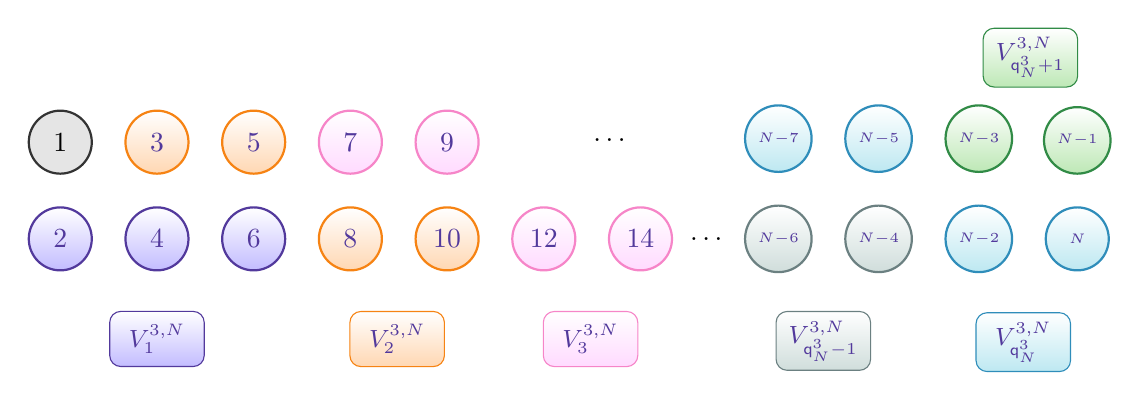
\begin{tikzpicture}
\tikzstyle{main}=[circle, minimum size = 8mm, thick, draw =black!80, node distance = 4mm]
\tikzstyle{V6}=[draw =black!80,circle,minimum size = 8mm, thick,node distance = 4mm,palegreen,bottom color=palegreen!30,top color= white, text=violet]
\tikzstyle{V5}=[draw =black!80,circle,minimum size = 8mm, thick,node distance = 4mm,burntblue,bottom color=burntblue!30,top color= white, text=violet]
\tikzstyle{V4}=[draw =black!80,circle,minimum size = 8mm, thick,node distance = 4mm,burntgreen,bottom color=burntgreen!30,top color= white, text=violet]
\tikzstyle{V3}=[draw =black!80,circle,minimum size = 8mm, thick,node distance = 4mm,lavander,bottom color=lavander!30,top color= white, text=violet]
\tikzstyle{V2}=[draw =black!80,circle,minimum size = 8mm, thick,node distance = 4mm,burntorange,bottom color=burntorange!30,top color= white, text=violet]
\tikzstyle{V1}=[draw =black!80,circle,minimum size = 8mm, thick,node distance = 4mm,violet,bottom color=violet!30,top color= white, text=violet]

\tikzstyle{legend_V1}=[node distance = 5mm,rectangle, rounded corners, thin,bottom color=violet!30, ,top color= white,
                           violet, fill= white, draw, text=violet,
                           minimum width=1.2cm, minimum height=0.7cm]
\tikzstyle{legend_V2}=[node distance = 8.8mm,rectangle, rounded corners, thin,bottom color=burntorange!30, ,top color= white,
                           burntorange, fill= white, draw, text=violet,
                           minimum width=1.2cm, minimum height=0.7cm]
\tikzstyle{legend_V3}=[node distance = 8.8mm,rectangle, rounded corners, thin,bottom color=lavander!30, ,top color= white,
                           lavander, fill= white, draw, text=violet,
                           minimum width=1.2cm, minimum height=0.7cm]      
\tikzstyle{legend_V4}=[node distance = 8.8mm,rectangle, rounded corners, thin,bottom color=burntgreen!30, ,top color= white,
                           burntgreen, fill= white, draw, text=violet,
                           minimum width=1.2cm, minimum height=0.6cm]                                                                                 
\tikzstyle{legend_V5}=[node distance = 8.8mm,rectangle, rounded corners, thin,bottom color=burntblue!30, ,top color= white,
                           burntblue, fill= white, draw, text=violet,
                           minimum width=1.2cm, minimum height=0.6cm]     
\tikzstyle{legend_V6}=[node distance = 4.8mm,rectangle, rounded corners, thin,bottom color=palegreen!30, ,top color= white,
                           palegreen, fill= white, draw, text=violet,
                           minimum width=1.2cm, minimum height=0.6cm]                                                             
\tikzstyle{connect}=[-latex, thick]
\tikzstyle{box}=[rectangle, draw=black!100]
\node[main, fill = black!10] (v1){$1$ };
\node[V2] (v3) [right=of v1] {$3$ };
\node[V2] (v5) [right=of v3] {$5$ };
\node[V3] (v7) [right=of v5] {$7$ };
\node[V3] (v9) [right=of v7] {$9$ };
%\node[main] (v11) [right=of v9] {$11$ };
%\node[main] (v13) [right=of v11] {$13$ };
%\node[main] (v7) [right=of v5] {{\small$2i-1$}};
%\node[main] (v9) [right=of v7] {{\small$N-5$}};
%\node[main] (v11) [right=of v9] {{\small$N-3$}};
\node[V1] (v2) [below=of v1] {$2$};
\node[V1] (v4) [below=of v3] {$4$};
\node[V1] (v6) [below=of v5] {$6$};
\node[V2] (v8) [below=of v7] {$8$};
\node[V2] (v10) [below=of v9] {$10$};
\node[V3] (v12) [right=of v10] {$12$};
\node[V3] (v14) [right=of v12] {$14$};
\node[V4] (v16) [right=of v14,xshift= .5cm] {${\scriptscriptstyle N-6}$};
\node[V4] (v18) [right=of v16] {${\scriptscriptstyle N-4}$};
\node[V5] (v20) [right=of v18] {${\scriptscriptstyle N-2}$};
\node[V5] (v22) [right=of v20] {${\scriptscriptstyle N}$};
\node[V5] (v11) [above=of v16] {${\scriptscriptstyle N-7}$};
\node[V5] (v13) [above=of v18] {${\scriptscriptstyle N-5}$};
\node[V6] (v15) [above=of v20] {${\scriptscriptstyle N-3}$};
\node[V6] (v17) [above=of v22] {${\scriptscriptstyle N-1}$};
%\node[main] (v8) [below=of v7] {{\small$2i$}};
%\node[main] (v10) [below=of v9] {{\small$N$}};
%\node[main] (v12) [below=of v11] {{\small$N-1$}};
%\draw (v1) -- (v2);
%\draw (v3) -- (v4);
%\draw (v5) -- (v6);
%\draw (v7) -- (v8);
%\draw (v9) -- (v10);  
%\draw (v11) -- (v12);     
\path (v14) -- node[auto=false]{\ldots}  (v16); 
\path (v9) -- node[auto=false]{\ldots}  (v11); 
%\path (v7) -- node[auto=false]{\ldots}  (v9); 
%\path (v6) -- node[auto=false]{\ldots}  (v8); 
%\path (v8) -- node[auto=false]{\ldots}  (v10);    
\node[legend_V1] [below=of v4] {\small{\textsc{$V_1^{3,N}$}}};
\node[legend_V2] [below right=of v6,xshift= .3cm] {\small{\textsc{$V_2^{3,N}$}}};
\node[legend_V3] [below right=of v10,xshift= .3cm] {\small{\textsc{$V_3^{3,N}$}}};
\node[legend_V4] [below right=of v14,xshift= .8cm] {\small{\textsc{$V_{\ordermax{3}{N}-1}^{3,N}$}}};
\node[legend_V5] (leg) [below right=of v18,xshift= .3cm] {\small{\textsc{$V_{\ordermax{3}{N}}^{3,N}$}}};
\node[legend_V6] [above right =of v15,xshift= -.6cm] {\small{\textsc{$V_{\ordermax{3}{N}+1}^{3,N}$}}};
\end{tikzpicture}
\caption{Elements of $\cV^{3,N}$, case $\remainder{3}{N} = 0$.}
\label{fig:groups:r0}
\end{figure}

\begin{figure}[h!]
\centering
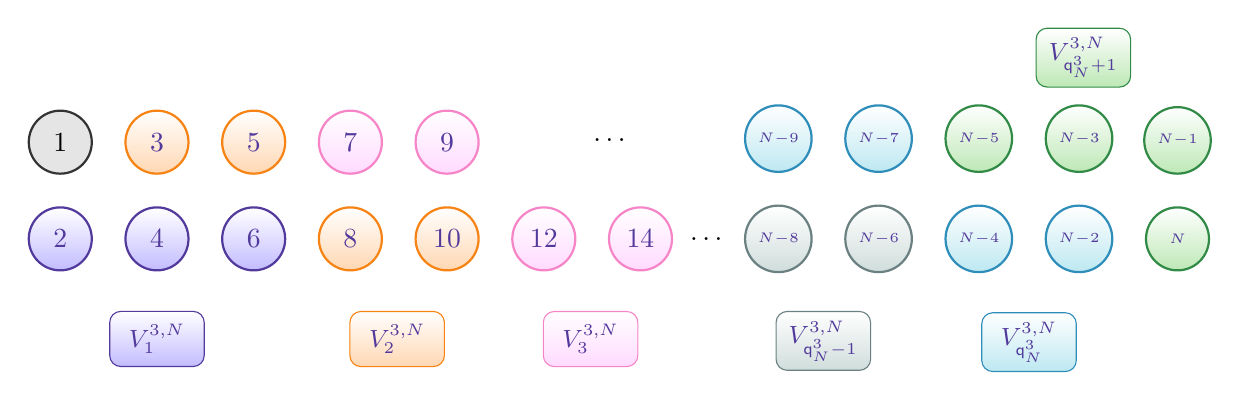
\begin{tikzpicture}
\tikzstyle{main}=[circle, minimum size = 8mm, thick, draw =black!80, node distance = 4mm]
\tikzstyle{V6}=[draw =black!80,circle,minimum size = 8mm, thick,node distance = 4mm,palegreen,bottom color=palegreen!30,top color= white, text=violet]
\tikzstyle{V5}=[draw =black!80,circle,minimum size = 8mm, thick,node distance = 4mm,burntblue,bottom color=burntblue!30,top color= white, text=violet]
\tikzstyle{V4}=[draw =black!80,circle,minimum size = 8mm, thick,node distance = 4mm,burntgreen,bottom color=burntgreen!30,top color= white, text=violet]
\tikzstyle{V3}=[draw =black!80,circle,minimum size = 8mm, thick,node distance = 4mm,lavander,bottom color=lavander!30,top color= white, text=violet]
\tikzstyle{V2}=[draw =black!80,circle,minimum size = 8mm, thick,node distance = 4mm,burntorange,bottom color=burntorange!30,top color= white, text=violet]
\tikzstyle{V1}=[draw =black!80,circle,minimum size = 8mm, thick,node distance = 4mm,violet,bottom color=violet!30,top color= white, text=violet]

\tikzstyle{legend_V1}=[node distance = 5mm,rectangle, rounded corners, thin,bottom color=violet!30, ,top color= white,
                           violet, fill= white, draw, text=violet,
                           minimum width=1.2cm, minimum height=0.7cm]
\tikzstyle{legend_V2}=[node distance = 8.8mm,rectangle, rounded corners, thin,bottom color=burntorange!30, ,top color= white,
                           burntorange, fill= white, draw, text=violet,
                           minimum width=1.2cm, minimum height=0.7cm]
\tikzstyle{legend_V3}=[node distance = 8.8mm,rectangle, rounded corners, thin,bottom color=lavander!30, ,top color= white,
                           lavander, fill= white, draw, text=violet,
                           minimum width=1.2cm, minimum height=0.7cm]      
\tikzstyle{legend_V4}=[node distance = 8.8mm,rectangle, rounded corners, thin,bottom color=burntgreen!30, ,top color= white,
                           burntgreen, fill= white, draw, text=violet,
                           minimum width=1.2cm, minimum height=0.6cm]                                                                                 
\tikzstyle{legend_V5}=[node distance = 8.8mm,rectangle, rounded corners, thin,bottom color=burntblue!30, ,top color= white,
                           burntblue, fill= white, draw, text=violet,
                           minimum width=1.2cm, minimum height=0.6cm]     
\tikzstyle{legend_V6}=[node distance = 4.8mm,rectangle, rounded corners, thin,bottom color=palegreen!30, ,top color= white,
                           palegreen, fill= white, draw, text=violet,
                           minimum width=1.2cm, minimum height=0.6cm]                                                             
\tikzstyle{connect}=[-latex, thick]
\tikzstyle{box}=[rectangle, draw=black!100]
\node[main, fill = black!10] (v1){$1$} ;
\node[V2] (v3) [right=of v1] {$3$};
\node[V2] (v5) [right=of v3] {$5$};
\node[V3] (v7) [right=of v5] {$7$};
\node[V3] (v9) [right=of v7] {$9$};
%\node[main] (v11) [right=of v9] {$11$ };
%\node[main] (v13) [right=of v11] {$13$ };
%\node[main] (v7) [right=of v5] {{\small$2i-1$}};
%\node[main] (v9) [right=of v7] {{\small$N-5$}};
%\node[main] (v11) [right=of v9] {{\small$N-3$}};
\node[V1] (v2) [below=of v1] {$2$};
\node[V1] (v4) [below=of v3] {$4$};
\node[V1] (v6) [below=of v5] {$6$};
\node[V2] (v8) [below=of v7] {$8$};
\node[V2] (v10) [below=of v9] {$10$};
\node[V3] (v12) [right=of v10] {$12$};
\node[V3] (v14) [right=of v12] {$14$};
\node[V4] (v24) [right=of v14,xshift= .5cm] {${\scriptscriptstyle N-8}$};
\node[V4] (v16) [right=of v24] {${\scriptscriptstyle N-6}$};
\node[V5] (v18) [right=of v16] {${\scriptscriptstyle N-4}$};
\node[V5] (v20) [right=of v18] {${\scriptscriptstyle N-2}$};
\node[V6] (v22) [right=of v20] {${\scriptscriptstyle N}$};
\node[V5] (v19) [above=of v24] {${\scriptscriptstyle N-9}$};
\node[V5] (v11) [above=of v16] {${\scriptscriptstyle N-7}$};
\node[V6] (v13) [above=of v18] {${\scriptscriptstyle N-5}$};
\node[V6] (v15) [above=of v20] {${\scriptscriptstyle N-3}$};
\node[V6] (v17) [above=of v22] {${\scriptscriptstyle N-1}$};
%\node[main] (v8) [below=of v7] {{\small$2i$}};
%\node[main] (v10) [below=of v9] {{\small$N$}};
%\node[main] (v12) [below=of v11] {{\small$N-1$}};
%\draw (v1) -- (v2);
%\draw (v3) -- (v4);
%\draw (v5) -- (v6);
%\draw (v7) -- (v8);
%\draw (v9) -- (v10);  
%\draw (v11) -- (v12);     
\path (v14) -- node[auto=false]{\ldots}  (v24); 
\path (v9) -- node[auto=false]{\ldots}  (v19); 
%\path (v7) -- node[auto=false]{\ldots}  (v9); 
%\path (v6) -- node[auto=false]{\ldots}  (v8); 
%\path (v8) -- node[auto=false]{\ldots}  (v10);    
\node[legend_V1] [below=of v4] {\small{\textsc{$V_1^{3,N}$}}};
\node[legend_V2] [below right=of v6,xshift= .3cm] {\small{\textsc{$V_2^{3,N}$}}};
\node[legend_V3] [below right=of v10,xshift= .3cm] {\small{\textsc{$V_3^{3,N}$}}};
\node[legend_V4] [below right=of v14,xshift= .8cm] {\small{\textsc{$V_{\ordermax{3}{N}-1}^{3,N}$}}};
\node[legend_V5] (leg) [below right=of v18,xshift= -.9cm] {\small{\textsc{$V_{\ordermax{3}{N}}^{3,N}$}}};
\node[legend_V6] [above right =of v15,xshift= -1.2cm] {\small{\textsc{$V_{\ordermax{3}{N}+1}^{3,N}$}}};
\end{tikzpicture}
\caption{Elements of $\cV^{3,N}$, case $\remainder{3}{N} = 1$.}
\label{fig:groups:r1}
\end{figure}


\begin{figure}[h!]
\centering
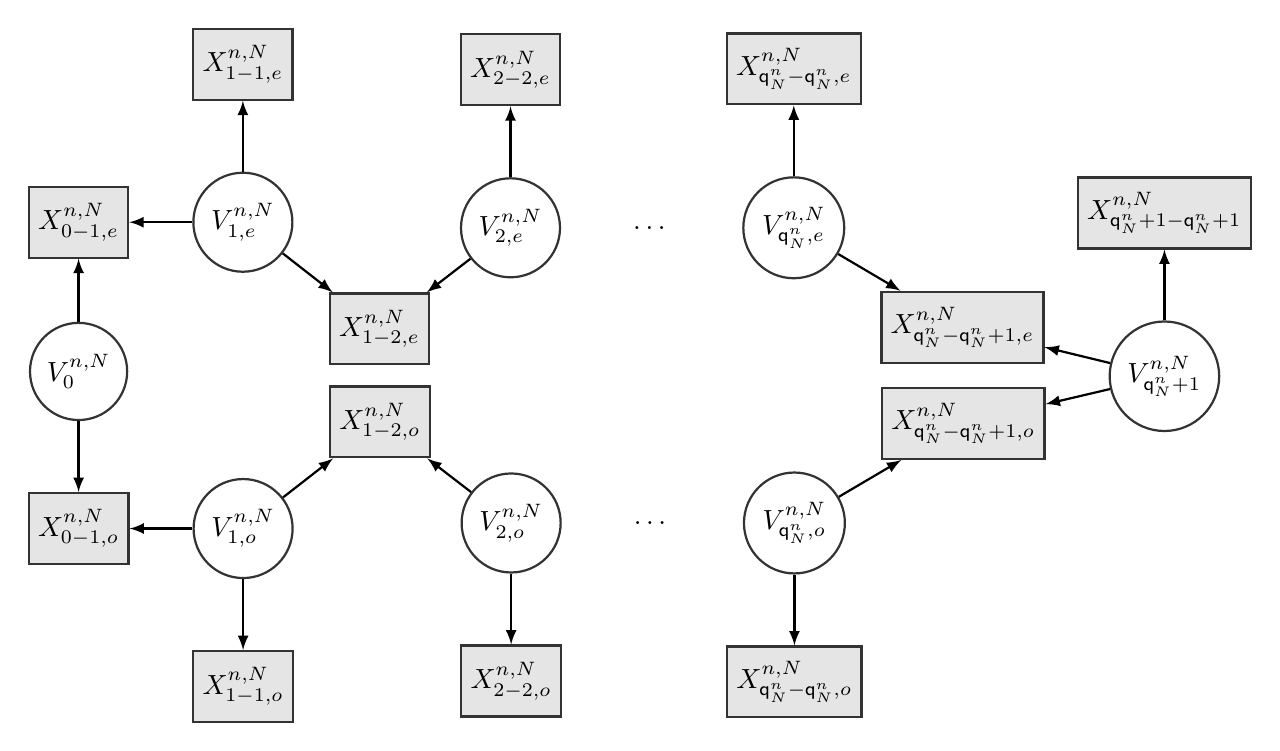
\begin{tikzpicture}
\tikzstyle{player}=[circle, minimum size = 9mm, thick, draw =black!80, node distance = 8mm]
\tikzstyle{game}=[rectangle, minimum size = 9mm, thick, draw =black!80, node distance = 9mm]
\tikzstyle{connect}=[-latex, thick]
\tikzstyle{box}=[rectangle, draw=black!100]
\node[game, fill = black!10] (v1){$X^{n,N}_{0-1,e}$};
\node[player] (v2) [below=of v1] {$V^{n,N}_{0}$};
\node[game, fill = black!10] (v3) [below=of v2] {$X^{n,N}_{0-1,o}$};
\node[player] (v4) [right=of v1] {$V^{n,N}_{1,e}$ };
\node[player] (v5) [right=of v3] {$V^{n,N}_{1,o}$ };
\node[game, fill = black!10] (v6) [above=of v4] {$X^{n,N}_{1-1,e}$};
\node[game, fill = black!10] (v7) [below=of v5] {$X^{n,N}_{1-1,o}$};

\path (v2) edge [connect] (v3);  
\path (v2) edge [connect] (v1);  
\path (v4) edge [connect] (v1);  
\path (v4) edge [connect] (v6);  
\path (v5) edge [connect] (v3);  
\path (v5) edge [connect] (v7);  

\node[game, fill = black!10] (v8) [below right =of v4,yshift=+.2cm] {$X^{n,N}_{1-2,e}$};
\node[game, fill = black!10] (v9) [above right =of v5,yshift=-.2cm] {$X^{n,N}_{1-2,o}$};
\node[player] (v10) [above right=of v8,yshift=-.2cm] {$V^{n,N}_{2,e}$};
\node[player] (v11) [below right=of v9,yshift=+.2cm] {$V^{n,N}_{2,o}$};
\node[game, fill = black!10] (v12) [above=of v10] {$X^{n,N}_{2-2,e}$};
\node[game, fill = black!10] (v13) [below=of v11] {$X^{n,N}_{2-2,o}$};

\path (v10) edge [connect] (v12);  
\path (v10) edge [connect] (v8);  
\path (v11) edge [connect] (v13);  
\path (v11) edge [connect] (v9);  
\path (v4) edge [connect] (v8);  
\path (v5) edge [connect] (v9);  

\node[player] (v14) [right=of v10,xshift=1.5cm] {$V^{n,N}_{\ordermax{n}{N},e}$};
\node[player] (v15) [right=of v11,xshift=1.5cm] {$V^{n,N}_{\ordermax{n}{N},o}$};

\path (v10) -- node[auto=false]{\ldots}  (v14); 
\path (v11) -- node[auto=false]{\ldots}  (v15); 

\node[game, fill = black!10] (v16) [above=of v14] {$X^{n,N}_{\ordermax{n}{N}-\ordermax{n}{N},e}$};
\node[game, fill = black!10] (v17) [below=of v15] {$X^{n,N}_{\ordermax{n}{N}-\ordermax{n}{N},o}$};

\path (v14) edge [connect] (v16);  
\path (v15) edge [connect] (v17);  

%\node[game, fill = black!10] (v18) [below left=of v14] {$X^{n,N}_{\ordermax{n}{N}-1-\ordermax{n}{N},e}$};
\node[game, fill = black!10] (v18) [below right=of v14,yshift=.3cm] {$X^{n,N}_{\ordermax{n}{N}-\ordermax{n}{N}+1,e}$};
\node[game, fill = black!10] (v19) [above right=of v15,yshift=-.3cm] {$X^{n,N}_{\ordermax{n}{N}-\ordermax{n}{N}+1,o}$};

\path (v14) edge [connect] (v18);  
\path (v15) edge [connect] (v19);  

\node[player] (v20) [right=of v19,yshift=.6cm] {$V^{n,N}_{\ordermax{n}{N}+1}$};

\path (v20) edge [connect] (v18);  
\path (v20) edge [connect] (v19); 

\node[game, fill = black!10] (v21) [above=of v20] {$X^{n,N}_{\ordermax{n}{N}+1-\ordermax{n}{N}+1}$};

\path (v20) edge [connect] (v21); 

%\node[player] (v5) [right=of v3] {$5$ };
%\node[player] (v7) [right=of v5] {${\scriptscriptstyle 2i-1}$};
%\node[player] (v9) [right=of v7] {${\scriptscriptstyle N-3}$};
%\node[player] (v11) [right=of v9] {${\scriptscriptstyle N-1}$};
%
%\node[player] (v4) [below=of v3] {$4$};
%\node[player] (v6) [below=of v5] {$6$};
%\node[player] (v8) [below=of v7] {${\scriptscriptstyle 2i}$};
%\node[player] (v10) [below=of v9] {${\scriptscriptstyle N-2}$};
%\node[player] (v12) [below=of v11] {${\scriptscriptstyle N}$};
%\path (v2) edge [connect] (v3);   
%\path (v4) edge [connect] (v2);  
%\path (v3) edge [connect] (v5);  
%\path (v6) edge [connect] (v4); 
%\path (v9) edge [connect] (v11); 
%\path (v11) edge [connect] (v12);   
%\path (v12) edge [connect] (v10);   
%\path (v5) -- node[auto=false]{\ldots}  (v7); 
%\path (v7) -- node[auto=false]{\ldots}  (v9); 
%\path (v6) -- node[auto=false]{\ldots}  (v8); 
%\path (v8) -- node[auto=false]{\ldots}  (v10);    
\end{tikzpicture}
\caption{Graphical model of the Round-robin algorithm.}
\label{fig:robin:graphicalmodel}
\end{figure}

\subsubsection{Elements of $\cX^{n,N}$}

Let us first build 
\[
X_{0-1,e}^{n,N}=\{X_{1,4x} : x=1,\ldots,\PE{n/2}\}=\{X_{1,i} : v_i\in V_{1,e}^{n,N}\},\qquad X_{0-1,o}^{n,N}=\{X_{1,i} : v_i\in V_{1,o}^{n,N}\}\enspace.
\]
In words, for any $X_{i,j}\in X_{0-1,o}^{n,N}$, $X_{i,j}$ denotes the result of the game of $v_1$ (that is of all elements of $V_{0}^{n,N}$) against its opponent (in $V_{1}^{n,N}$) at time $t$ when $t$ is odd. Let us now describe the games involving players in $V_{1}^{n,N}$ against opponents that are both differents from $1$. Start with the games between players in $V_{1}^{n,N}$ and let 
\begin{gather*}
X_{1-1,e}^{n,N}=\{X_{4x,4y} : (x,y)\in [\PE{n/2}], x< y\}=\{X_{i,j} : v_i,v_j\in V_{1,e}^{n,N},i<j\}\enspace,\\
X_{1-1,o}^{n,N}=\{X_{i,j} : v_i,v_j\in V_{1,o}^{n,N},i<j\}\enspace. 
\end{gather*}
One can check that there is no game between any $v_i\in V_{1,e}^{n,N}$ and an opponent $v_j\in V_{q,o}^{n,N}$ for any $q\ge 1$. 
%The same property holds if we reverse the roles of $e$ and $o$. 
In particular there is no game between any $v_i\in V_{1,e}^{n,N}$ and an opponent $v_j\in V_{1,o}^{n,N}$.  Therefore, $X_{1-1,e}^{n,N}\cup X_{1-1,o}^{n,N}$ describes all games between players in $V_{1}^{n,N}$. 

Let us now describe the games between $i\in V_{1}^{n,N}$ and $j\in V_{2}^{n,N}$. Let 
\begin{align*}
&X_{1-2,e}^{n,N}=\{X_{4y-1-4k,4y} : y\in [\PE{n/2}], k<y\}\cup\{X_{4x,4y} : x\in[\PE{n/4}], y\in[\PE{n/2}+1,n-x]\}\\
&=\{X_{i,j} : v_i\in V_{1,e}^{n,N},v_j\in V_{2,e}^{n,N},j\in 2\bZ+1,j>i\}\cup\{X_{i,j} : v_i\in V_{1,e}^{n,N},v_j\in V_{2,e}^{n,N},j\in 2\bZ\cap [4n-i]\}\enspace,\\
&X_{1-2,o}^{n,N}=\{X_{i,j} : v_i\in V_{1,o}^{n,N},v_j\in V_{2,o}^{n,N},j\in 2\bZ+1,j>i\}\cup\{X_{i,j} : v_i\in V_{1,o}^{n,N},v_j\in V_{2,o}^{n,N},j\in 2\bZ\cap [4n-i]\}\enspace.
\end{align*}
Again these are all games between a $v_i\in V_{1}^{n,N}$ and $v_j\in V_{2}^{n,N}$.

Now, for any $q\in [2,\ordermax{n}{N}]$, we can describe the games between players $i$ and $j$ both in $V_{q}^{n,N}$. One can use \eqref{eq:Opponents} to check that
\begin{align}
 \notag X_{q- q,e}^{n,N}&=\{X_{i,j} : v_i\in V_{q,e}^{n,N},i\in 2\bZ+1, v_j\in V_{q,e}^{n,N},j\in 2\bZ\}\enspace,\\
\label{Def:Vqtoq}  X_{q- q,o}^{n,N}&=\{X_{i,j} : v_i\in V_{q,o}^{n,N},i\in 2\bZ+1, v_j\in V_{q,o}^{n,N},j\in 2\bZ\}\enspace.
\end{align}
Eq~\eqref{eq:Opponents} shows also that there is no game between $v_i\in V_{q,e}^{n,N}$ and $v_j\in V_{q,o}^{n,N}$. 

Let us give the games between a player $v_i\in V_{q}^{n,N}$ and a $v_j\in V_{q+1}^{n,N}$, for all $q\in[2,\ordermax{n}{N}-1]$.
\begin{align*}
X_{q- q+1,e}^{n,N}=&\{X_{i,j} : v_i\in V_{q,e}^{n,N},i\in(2\bZ+1),v_j\in V_{q+1,e}^{n,N}j\in 2\bZ\cap [i+4n-3]\}\\
&\cup\{X_{i,j} : v_i\in V_{q,e}^{n,N},i\in 2\bZ,v_j\in V_{q+1,e}^{n,N},j\in 2\bZ+1\cap [i]\}\enspace,\\
X_{q- q+1,o}^{n,N}=&\{X_{i,j} : v_i\in V_{q,o}^{n,N},i\in(2\bZ+1),v_j\in V_{q+1,o}^{n,N},j\in2\bZ\cap [i+4n-3]\}\\
&\cup\{X_{i,j} : v_i\in V_{q,o}^{n,N},i\in2\bZ,v_j\in V_{q+1,o}^{n,N},j\in( 2\bZ+1)\cap [i]\}\enspace.
\end{align*}

\subsubsection{Cardinality of the cells}
It is easy to check that 
\[
|V_{0}^{n,N}|=1, \qquad |V_{1}^{n,N}|=n,\qquad |V_{q}^{n,N}|=2(n-1),\qquad\forall q\in[2,\ordermax{n}{N}]\enspace,
\]
furthermore, one also has
\[
|V_{q,e}^{n,N}|=|V_{q,o}^{n,N}|=n-1,\qquad \forall q\in [2,\ordermax{n}{N}]\enspace.
\]
Finally either $n-1=2p$, for some $p\in \bN$ and, in this case 
\[
|\{j: v_j\in V_{q,e}^{n,N},j\in 2\bZ\}|=|\{i : v_i\in V_{q,e}^{n,N},i\in 2\bZ+1\}|=p\enspace,
\]
or $n-1=2p+1$ for some $p\in \bN$ and, in this case either 
\[
|\{j: v_j\in V_{q,e}^{n,N},j\in 2\bZ\}|=p,\qquad\text{and}\qquad |\{i : v_i\in V_{q,e}^{n,N},i\in 2\bZ+1\}|=p+1\enspace,
\]
or 
\[
|\{j: v_j\in V_{q,e}^{n,N},j\in 2\bZ\}|=p+1,\qquad\text{and}\qquad |\{i : v_i\in V_{q,e}^{n,N},i\in 2\bZ+1\}|=p\enspace.
\]
Now,
\begin{align*}
|X_{q- q,e}^{n,N}|&=|\{i : v_i\in V_{q,e}^{n,N},i\in 2\bZ+1\}||\{j: v_j\in V_{q,e}^{n,N},j\in 2\bZ\}|\\
&=
\begin{cases}
 p^2&\text{ if }n-1=2p\\
 p(p+1)&\text{ if }n-1=2p+1
\end{cases}
\enspace. 
\end{align*}
\begin{align*}
|X_{q- q+1,e}^{n,N}|=&\sum_{i : v_i\in V_{q,e}^{n,N},i\in(2\bZ+1)}|\{j : v_j\in V_{q+1,e}^{n,N}j\in 2\bZ\cap [i+4n-3]\}\\
&+\sum_{i : v_i\in V_{q,e}^{n,N},i\in 2\bZ}|\{j: v_j\in V_{q+1,e}^{n,N},j\in 2\bZ+1\cap [i]\}|\\
&=
\begin{cases}
2\sum_{i=1}^pi=p(p+1) &\text{ if }n-1=2p\\
\sum_{i=1}^pi+\sum_{i=1}^{p+1}i=(p+1)^2 &\text{ if }n-1=2p+1
\end{cases}
\enspace.
\enspace,
\end{align*}

\subsection{Bounding the kernel}
%For all $n,N$ define $\ordermax{n}{N}$ by:
%\begin{equation}
%\label{eq:ordermax}
%\ordermax{n}{N} = \max\left\{q\ge 1;\eqsp n+1 + 2(q-1)(n-1)\le N\right\}\eqsp.
%\end{equation}
%The log-likelihood defined by \eqref{eq:def:loglik} may be written $\Lo{\cD_{n,N}}{\pi}= -\log p_{\pi}^{n,N}\left(\cD_{n,N}\right)$,
%where $p^{n,N}$ is the joint likelihood of the observations:
%\[
%p_{\pi}^{n,N}\left(\cD_{n,N}\right) = \int \prod_{(i,j)\in A_{n,N}}k(X_{i,j},v_{\{i,j\}})\pi^{\otimes N}(\rmd v) \eqsp.
%\]
Consider the following notations, for $0\le q \le \ordermax{n}{N}-1$,
\begin{align*}
%X_{0}^{n,N} & = X_{0-1,e}^{n,N}\cup X_{1-1,e}^{n,N}\cup X_{0-1,o}^{n,N}\cup X_{1-1,e}^{n,N}\eqsp,\\
X_{q}^{n,N}                   & = X_{q- q+1,e}^{n,N}\cup X_{q+1-q+1,e}^{n,N}\cup X_{q-q+1,o}^{n,N}\cup X_{q+1 - q+1,o}^{n,N}\eqsp,\\
X^{n,N}_{q- q+1} &= X^{n,N}_{q- q+1,e}\cup X^{n,N}_{q- q+1,o}\eqsp,\\
X_{\ordermax{n}{N}}^{n,N} = X_{\ordermax{n}{N}-\ordermax{n}{N}+1}^{n,N} & = X_{\ordermax{n}{N} - \ordermax{n}{N} +1,e}^{n,N}\cup X_{\ordermax{n}{N}+1-\ordermax{n}{N}+1}^{n,N}\cup X_{\ordermax{n}{N}-\ordermax{n}{N}+1,o}^{n,N}\eqsp.
\end{align*}
The loglikelihood of the observations may be decomposed as follows:
\[
\log p_{\pi}^{n,N}\left(X_{\cA_{n,N}}\right) = \log p_{\pi}^{n,N}\left(X_{\ordermax{n}{N}}^{n,N}\right) + \sum_{q=1}^{\ordermax{n}{N}-1}  \log p_{\pi}^{n,N}\left(X_{q}^{n,N}\middle|X_{q+1:\ordermax{n}{N}}^{n,N}\right) +  \log p_{\pi}^{n,N}\left(X_{0}^{n,N}\middle|X_{1:\ordermax{n}{N}}^{n,N}\right)\eqsp.
\]
This section extends the analysis of the asymptotic properties of the maximum likelihood estimator to Bradley-Terry models in random environment. For all $1\le q \le \ordermax{n}{N}$, this asymptotic behavior is established using the geometric decaying mixing rate of the conditional law of the $(V^{n,N}_{k})_{q< k < \ordermax{n}{N}}$ given the observations $X^{n,N}_{q+1:\ordermax{n}{N}}$ which is based on the graphical model displayed in Figure~\ref{fig:robin:graphicalmodel}.
%\begin{align*}
%X_{\mathsf{beg}}^{n,N} & = \left\{X_{i,j};\;(i,j)\in V_{g,u\to u+1,e}^{n,N}\cup V_{g,u+1\to u+1,e}^{n,N}\cup V_{g,u\to u+1,o}^{n,N}\cup V_{g,u+1\to u+1,o}^{n,N},\;0\le u\le 1\right\}\eqsp,\\
%X_{q}^{n,N}                   & = \left\{X_{i,j};\;(i,j)\in V_{g,q\to q+1,e}^{n,N}\cup V_{g,q+1\to q+1,e}^{n,N}\cup V_{g,q\to q+1,o}^{n,N}\cup V_{g,q+1\to q+1,o}^{n,N}\right\} \eqsp,\\
%X_{\mathsf{end}}^{n,N} & = X_{\cA_{n,N}}\setminus (X_{\mathsf{beg}}^{n,N}\cup\cup_{q=2}^{\ordermax{n}{N}} X_{q}^{n,N} )\eqsp.
%\end{align*}
This mixing rate is obtained under the following assumption.
\begin{hypH}
\label{assum:strongmix}
There exists $\varepsilon>0$ such that for all $x\in\{0,1\}$, all $\pi\in\Pi$ and all $v_1,v_2 \in \mathrm{supp}(\pi)$ , 
\begin{equation}
\label{eq:bound:likelihood}
\varepsilon(1+\varepsilon)^{-1}\le \condlik(x,v_{\{1,2\}})\le 1\eqsp.
\end{equation}
\end{hypH}
Note that the forgetting properties established in this section are consequences of the graphical model given in Figure~\ref{fig:robin:graphicalmodel} and of the boundedness assumption H\ref{assum:strongmix} of the conditional likelihood of the observations. Therefore, the results of this section hold for any model describing the outcomes of paired comparisons where the 'players' meet according to the round-robin scheduling if the conditional likelihood of the observations are bounded above and away from from zero. They hold in particular in the following cases.
\begin{enumerate}[-]
\item {\em Bradley-Terry model}: when the function $\condlik$ is given by \eqref{eq:def:condlik} if for all $\pi \in\Pi$, $\mathrm{supp}(\pi) \subset (1,\varepsilon]$.
\item \textcolor{red}{Other models}.
\end{enumerate}



%consequence of the fact that the support of all probability densities in $\Pi$ is included in $(\varepsilon,1]$ which implies that for all $x\in\{0,1\}$, all $\pi\in\Pi$ and all $v_1,v_2 \in \mathrm{supp}(\pi)$ , 
%\begin{equation}
%\label{eq:bound:likelihood}
%\varepsilon(1+\varepsilon)^{-1}\le \condlik(x,v_{\{1,2\}})\le 1\eqsp.
%\end{equation}
%Consider the following additional assumption on the model.
%\begin{hypH}
%\label{assum:strongmix}
%There exist $0<\sigma_-<\sigma_+<\infty$ such that for all $\pi\in\Pi$ and all $v\in [\varepsilon,1]$, $\sigma_-\le \pi(v)\le\sigma_+$.
%\end{hypH}

\begin{lemma}
\label{lem:minorization}
Assume that H\ref{assum:strongmix} holds. Then, for all $n,N$, $q\ge 1$, and all $\pi\in\Pi$, conditionally on the observations $(X_{q+1:\ordermax{n}{N}}^{n,N})$, $(V_{\ordermax{n}{N}}^{n,N},\ldots,V_q^{n,N})$ is a Markov chain.
% chain with transition kernel given, 
% for all $1\le q \le \ordermax{n}{N}$ and all measurable set $A$:
%%\[
%%\mathbb{P}\left(V^{n,N}_{p,\ordermax{n}{N}}\in A\middle|V^{n,N}_{p,\mathsf{end}},X_{2:\ordermax{n}{N}}^{n,N},X_{\mathsf{end}}^{n,N}\right) = 
%%\]
%\[
%\mathbb{P}_{\pi}\left(V^{n,N}_{q}\in A\middle|V^{n,N}_{q+1:\ordermax{n}{N}+1},X_{2:\ordermax{n}{N}}^{n,N}\right) = \mathbb{P}_{\pi}\left(V^{n,N}_{q}\in A\middle|V^{n,N}_{q+1},X^{n,N}_{2:q-1},X^{n,N}_{q- q+1}\right)\eqsp.
%\]
In addition,  the transition kernels $(\kernel^{n,N}_{\pi,k,q})_{q< k <\ordermax{n}{N}}$ are such that, for all $q< k < \ordermax{n}{N}$, there exists a measure $\mu^{n,N}_{\pi,k,q}$ satisfying for all measurable set $A$:
\begin{align*}
\kernel^{n,N}_{\pi,k,q}(V^N_{k+1},A) = \mathbb{P}_{\pi}\left(V^{n,N}_{k}\in A\middle|V^{n,N}_{k+1:\ordermax{n}{N}},X_{q+1:\ordermax{n}{N}}^{n,N}\right)  &= \mathbb{P}_{\pi}\left(V^{n,N}_{k}\in A\middle|V^{n,N}_{k+1},X_{q+1:\ordermax{n}{N}}^{n,N}\right)\eqsp,\\
&\ge \left(\frac{\varepsilon}{1+\varepsilon}\right)^{\card\left(X^{n,N}_{k- k+1}\right)} \mu^{n,N}_{\pi,k,q}(A)\eqsp.
\end{align*}
\end{lemma}
%By \eqref{eq:bound:likelihood}, Lemma~\ref{lem:minorization}
\begin{proof}
The Markov property is a direct consequence of the graphical model given in Figure~\ref{fig:robin:graphicalmodel}. Then, for all $n,N$, for all $q< k < \ordermax{n}{N}$ and all measurable set $A$:
\begin{align*}
\mathbb{P}\left(V^{n,N}_{k}\in A\middle|V^{n,N}_{k+1:\ordermax{n}{N}},X_{q+1:\ordermax{n}{N}}^{n,N}\right) &\\
 &\hspace{-3.2cm}= \mathbb{P}\left(V^{n,N}_{k}\in A\middle|V^{n,N}_{k+1},X^{n,N}_{q+1:k-1},X^{n,N}_{k- k+1}\right)\eqsp,\\
 &\hspace{-3.2cm}= \frac{\int \1_{A}(v^{n,N}_{k})\pi(\rmd v^{n,N}_{k})\prod_{X_{i,j}\in X^{n,N}_{k- k+1}}\condlik(X_{i,j},v_{\{i,j\}})p_{\pi}^{n,N}(X^{n,N}_{q+1:k-1}|v^{n,N}_{k})}{\int \pi(\rmd v^{n,N}_{k})\prod_{X_{i,j}\in X^{n,N}_{k- k+1}}\condlik(X_{i,j},v_{\{i,j\}})p_{\pi}^{n,N}(X^{n,N}_{q+1:k-1}|v^{n,N}_{k})}\eqsp,
\end{align*}
with the conventions $X_{q+1:q} = \emptyset$ and $p_{\pi}^{n,N}(X^{n,N}_{q+1:q}|v^{n,N}_{q+1})$ being the constant function which equals one. By \eqref{eq:bound:likelihood},
\[
\mathbb{P}\left(V^{n,N}_{k}\in A\middle|V^{n,N}_{k+1},X_{q+1:\ordermax{n}{N}}^{n,N}\right)
\ge \left(\frac{\varepsilon}{1+\varepsilon}\right)^{\card\left(X^{n,N}_{k- k+1}\right)}\frac{\int \1_{A}(\rmd v^{n,N}_{k})\pi(v^{n,N}_{k})p_{\pi}^{n,N}(X^{n,N}_{q+1:k-1}|v^{n,N}_{k})}{\int \pi(\rmd v^{n,N}_{k})p_{\pi}^{n,N}(X^{n,N}_{q+1:k-1}|v^{n,N}_{k})}\eqsp. 
\]
The proof is then completed by choosing:
\[
\mu^{n,N}_{\pi,k,q}(A) = \frac{\int \1_{A}(v^{n,N}_{k})\pi(\rmd v^{n,N}_{k})p_{\pi}^{n,N}(X^{n,N}_{q+1:k-1}|v^{n,N}_{k})}{\int \pi(\rmd v^{n,N}_{k})p_{\pi}^{n,N}(X^{n,N}_{q+1:k-1}|v^{n,N}_{k})}\eqsp. 
\]
\end{proof}
%\begin{hypH}
%\label{assum:compact}
%There exist $0<c_-<c_+<\infty$ such that for all $\param\in\param$, $C_{\param} \subset (c_-,c_+)$.
%\end{hypH}
%Define 
%\begin{equation}
%\label{eq:def:rho}
%\rho_n = 1- \left(\frac{\varepsilon\sigma_-}{(\varepsilon+1)\sigma_+}\right)^2\eqsp.
%\end{equation}
Lemma~\ref{lem:minorization} implies that for all $1\le q\le \ordermax{n}{N}$,
\begin{multline*}
p_{\pi}^{n,N}\left(X^{n,N}_{q}\middle|X^{n,N}_{q+1:\ordermax{n}{N}}\right) = \int p_{\pi}\left(\rmd v_{\ordermax{n}{N}}^{n,N}\middle | X^{n,N}_{q+1:\ordermax{n}{N}}\right) \prod_{k =\ordermax{n}{N}-1}^{q+1}\kernel^{n,N}_{\pi,k,q}(v_{k+1}^{n,N},\rmd v_k^{n,N})\\
\times\int \pi(\rmd v_q^{n,N})\prod_{X_{i,j}\in X_{q}^{n,N}}\condlik(X_{i,j},v_{\{i,j\}})\eqsp.
\end{multline*}
By Lemma~\ref{lem:minorization}, conditional on $X_{q+1:\ordermax{n}{N}}^{n,N}$, the backward Markov chain $(V_{\ordermax{n}{N}}^{n,N},\ldots,V_{q}^{n,N})$ admits the whole state space as a $1$-small set and the minorizing constant does not depend on the observations. Then, the asymptotic behavior of the normalized loglikelihood function may be analyzed by proving that, if $\ell>1$ additional players are involved in the contest, the influence of the "initial" distributions $p_{\pi}^{n,N}(\rmd v_{\ordermax{n}{N}}|X^{n,N}_{q+1:\ordermax{n}{N}})$ and $p_{\pi}^{n,N}(\rmd v_{\ordermax{n}{N}}|X^{n,N+\ell}_{q+1:\ordermax{n}{N+\ell}})$ vanishes exponentially fast by \cite{lindvall:1992}.

%  For all $1\le q \le \ordermax{n}{N}$, all distribution $\lambda$ on $(\varepsilon,1]^{\card(V_{\ordermax{n}{N}}^{n,N})}$ and all measurable set $A$ define:
%\begin{equation}
%\phi^{n,N}_{q,\lambda}(A) = \frac{\int \1_{A}(v_{q}^{n,N})\left\{\prod_{u=q}^{\ordermax{n}{N}}\prod_{X_{i,j}\in X^{n,N}_{u}}\condlik(X_{i,j},v_{\{i,j\}})\right\}\left\{\prod_{u=q}^{\ordermax{n}{N}-1}\pi(\rmd v^{n,N}_{u})\right\}\lambda(\rmd v^{n,N}_{\ordermax{n}{N}})}{\int \left\{\prod_{u=q}^{\ordermax{n}{N}}\prod_{X_{i,j}\in X^{n,N}_{u}}\condlik(X_{i,j},v_{\{i,j\}})\right\}\left\{\prod_{u=q}^{\ordermax{n}{N}-1}\pi(\rmd v^{n,N}_{u})\right\}\lambda(\rmd v^{n,N}_{\ordermax{n}{N}})}\eqsp.\label{eq:filt}\\
%\end{equation}
%Then, for all $1\le q \le \ordermax{n}{N}$, the conditional distribution of $V_{q}^{n,N}$ given $X_{q:\ordermax{n}{N}}^{n,N}$ may be written, for all measurable set $A$:
%\begin{align*}
%\bP\left(V_{q}^{n,N}\in A \middle | X_{q:\ordermax{n}{N}}^{n,N}\right) %= \frac{\int \1_{A}(v_{q}^{n,N})\left\{\prod_{u=q}^{\ordermax{n}{N}}\pi(\rmd v^{n,N}_{u})\prod_{X_{i,j}\in X^{n,N}_{u}}\condlik(X_{i,j},v_{\{i,j\}})\right\}\pi(\rmd v^{n,N}_{\mathsf{end}})\prod_{X_{i,j}\in X^{n,N}_{\mathsf{end}}}\condlik(X_{i,j},v_{\{i,j\}})}{\int \left\{\prod_{u=q}^{\ordermax{n}{N}}\pi(\rmd v^{n,N}_{u})\prod_{X_{i,j}\in X^{n,N}_{u}}\condlik(X_{i,j},v_{\{i,j\}})\right\}\pi(\rmd v^{n,N}_{\mathsf{end}})\prod_{X_{i,j}\in X^{n,N}_{\mathsf{end}}}\condlik(X_{i,j},v_{\{i,j\}})}\eqsp,\\
% = \phi^{n,N}_{q,\widetilde{\pi}}(A)\eqsp,
%\end{align*}
%where, 
%\begin{equation}
% \widetilde{\pi}_{\ordermax{n}{N}}^{n,N}(A) = \frac{\int \1_A(v_{\ordermax{n}{N}}^{n,N}) \pi(\rmd v_{\ordermax{n}{N}}^{n,N})\pi(\rmd v_{\ordermax{n}{N}+1}^{n,N})\prod_{X_{i,j}\in X^{n,N}_{\ordermax{n}{N}}}\condlik\left(X_{i,j};v_{\{i,j\}}\right)}{\int \pi(\rmd v_{\ordermax{n}{N}}^{n,N})\pi(\rmd v_{\ordermax{n}{N}+1}^{n,N})\prod_{X_{i,j}\in X^{n,N}_{\ordermax{n}{N}}}\condlik\left(X_{i,j};v_{\{i,j\}}\right)}\eqsp.\label{eq:lastdist}
% \end{equation}

%For all $1\le k < n$ and all probability density function $\lambda$ on $\bar C_{\param}$, denote by $\phi^{n,k}_{\lambda,\param}$ the probability density of the conditional distribution of $\bar v_k$ given $(\bar X_n,\ldots,\bar X_k)$ when the state $\bar v_{n+1}$ has probability density function $\lambda$ on $\bar C_{\param}$. Note that for all $1\le k \le n < m$,
%\begin{align*}
%\phi^{m,k}_{\lambda,\param}\left(\bar v_{k}\right) &= \frac{\int \lambda(\bar v_{m+1})\prod_{i = m}^k\bar G(\bar X_i; \bar v_{i+1},\bar v_i) \bar \pi_{\param}(\bar v_i)\mu(\rmd \bar v_{m+1:k+1})}{\int \lambda(\bar v_{m+1})\prod_{i = m}^k\bar G(\bar X_i; \bar v_{i+1},\bar v_i) \bar \pi_{\param}(\bar v_i)\mu(\rmd \bar v_{m+1:k})} = \phi^{n,k}_{\eta^{m,n}_{\lambda,\param},\param}\left(\bar v_{k}\right)\eqsp,
%\end{align*}
%where, $\eta^{m,n}_{\lambda,\param}$ is the probability density function defined on $\bar C_{\param}$ as:
%\[
%\eta^{m,n}_{\lambda,\param}: \bar v_{n+1} \mapsto \frac{\int \lambda(\bar v_{m+1})\bar G(\bar X_m; \bar v_{m+1},\bar v_m)\prod_{i = m}^{n+2} \bar \pi_{\param}(\bar v_i) \bar G(\bar X_{i-1}; \bar v_{i},\bar v_{i-1}) \mu(\rmd \bar v_{m+1:n+2})}{\int \lambda(\bar v_{m+1})\bar G(\bar X_m; \bar v_{m+1},\bar v_m)\prod_{i = m}^{n+2} \bar \pi_{\param}(\bar v_i) \bar G(\bar X_{i-1}; \bar v_{i},\bar v_{i-1}) \mu(\rmd \bar v_{m+1:n+1})}\eqsp.
%\]
%\[
%\widetilde{\pi}^{n,N}(A) = \frac{\int \1_A(v_{\ordermax{n}{N}}^{n,N}) \pi(\rmd v_{\ordermax{n}{N}}^{n,N})\pi(\rmd v_{\mathsf{end}}^{n,N})\prod_{X_{i,j}\in X^{n,N}_{\mathsf{end}}}\condlik\left(X_{i,j};v_{\{i,j\}}\right)}{\int \pi(\rmd v_{\ordermax{n}{N}}^{n,N})\pi(\rmd v_{\mathsf{end}}^{n,N})\prod_{X_{i,j}\in X^{n,N}_{\mathsf{end}}}\condlik\left(X_{i,j};v_{\{i,j\}}\right)}
%\]
%
%
%\begin{multline*}
%p_{\pi}^{n,N}\left(X_{q}^{n,N}\middle|X_{\mathsf{end}}^{n,N},X_{q+1:\ordermax{n}{N}}^{n,N}\right) \\
%= \frac{\int \prod_{u=q}^{\ordermax{n}{N}-1}\pi(\rmd v_u^{n,N})\prod_{X_{i,j}\in X^{n,N}_{q}}\condlik\left(X_{i,j};v_{\{i,j\}}\right)\pi(\rmd v_{\ordermax{n}{N}}^{n,N})\int \pi(\rmd v_{\mathsf{end}}^{n,N})\prod_{X_{i,j}\in X^{n,N}_{\mathsf{end}}}\condlik\left(X_{i,j};v_{\{i,j\}}\right)}{\int \prod_{u=q+1}^{\ordermax{n}{N}-1}\pi(\rmd v_u^{n,N})\prod_{X_{i,j}\in X^{n,N}_{q}}\condlik\left(X_{i,j};v_{\{i,j\}}\right)\pi(\rmd v_{\ordermax{n}{N}}^{n,N})\int \pi(\rmd v_{\mathsf{end}}^{n,N})\prod_{X_{i,j}\in X^{n,N}_{\mathsf{end}}}\condlik\left(X_{i,j};v_{\{i,j\}}\right)}\eqsp,
%\end{multline*}
%
%
%For all $2\le q < \ordermax{n}{N}$ and all probability density function $\lambda$ on $(\varepsilon,1]^{\card(V_{\mathsf{end}}^{n,N})}$, denote by $\phi^{n,N}_{q,\lambda}$ the probability density of the conditional distribution of $V_{q}^{n,N}$ given $(X_{q:\ordermax{n}{N}}^{n,N},X_{\mathsf{end}}^{n,N})$ when the state $V_{\mathsf{end}}^{n,N}$ has probability density function $\lambda$ on $(\varepsilon,1]^{\card(V_{\mathsf{end}}^{n,N})}$. 
%For all $\ell>1$, $\widetilde{V}_{\mathsf{end}}^{(n,N+\ell)}$ denotes all the players that do not belong to:
%\[
%(X_{\ordermax{n}{N}+1:\ordermax{n}{N+\ell}}^{(n,N+\ell)},X_{\mathsf{end}}^{(n,N+\ell)}) = (X_{q:\ordermax{n}{N}}^{n,N},X_{\mathsf{end}}^{n,N})
%\]
%Note that for all $\ell>1$,
%\begin{align*}
%\phi^{n,N+\ell}_{q,\lambda}\left(v_{q}^{n,N}\right) &= \frac{\int \prod_{u=q}^{\ordermax{n}{N+\ell}}\pi(v_{u})\pi(v_{\mathsf{end}})\rmd v^{}_{}}{\int} = \phi^{n,N}_{q,\eta^{n,N}_{\lambda,\ell}}\left(v_{q}^{n,N}\right)\eqsp,
%\end{align*}
%where, $\eta^{n,N}_{\lambda,\ell}$ is the probability density function defined on $(\varepsilon,1]^{\card(V_{\mathsf{end}}^{n,N})}$ as:
%\[
%\eta^{n,N}_{\lambda,\ell}: \bar v_{n+1} \mapsto \frac{\int \lambda(\bar v_{m+1})\bar G(\bar X_m; \bar v_{m+1},\bar v_m)\prod_{i = m}^{n+2} \bar \pi_{\param}(\bar v_i) \bar G(\bar X_{i-1}; \bar v_{i},\bar v_{i-1}) \mu(\rmd \bar v_{m+1:n+2})}{\int \lambda(\bar v_{m+1})\bar G(\bar X_m; \bar v_{m+1},\bar v_m)\prod_{i = m}^{n+2} \bar \pi_{\param}(\bar v_i) \bar G(\bar X_{i-1}; \bar v_{i},\bar v_{i-1}) \mu(\rmd \bar v_{m+1:n+1})}\eqsp.
%\]

\begin{lemma}
\label{lem:exp:forget}
For all $n,N$, $\pi\in\Pi$,
\begin{align}
\sup_{\pi\in\Pi}\left|\log p_{\pi}^{n,N}\left(X_{\ordermax{n}{N}}^{n,N}\right)\right|&\le \card\left(X_{\ordermax{n}{N}}^{n,N}\right)\log \left(1+\varepsilon^{-1}\right)\eqsp,\label{eq:bound:beg}\\
\sup_{\pi\in\Pi}\left|\log p_{\pi}^{n,N}\left(X_{0}^{n,N}\middle|X_{1:\ordermax{n}{N}}^{n,N}\right)\right|&\le \card\left(X_{0}^{n,N}\right)\log \left(1+\varepsilon^{-1}\right)\label{eq:bound:end}\eqsp.
\end{align}
In addition,  for all $\ell>1$,  $1\le q< \ordermax{n}{N}$ and all $\pi\in\Pi$,
\begin{multline}
\sup_{\pi\in\Pi}\left|\log p_{\pi}^{n,N}\left(X_{q}^{n,N}\middle|X_{q+1:\ordermax{n}{N}}^{n,N}\right) - \log p_{\pi}^{n,N+\ell}\left(X_{q}^{(n,N+\ell)}\middle|X_{q+1:\ordermax{n}{N+\ell}}^{n,N+\ell}\right) \right|\\
\leq \left(1+\varepsilon^{-1}\right)^{\card\left(X^{n,N}_{q}\right)}\prod_{k=q+1}^{\ordermax{n}{N}-1}\rho_k(\varepsilon) \eqsp,\label{eq:bound:forget}
\end{multline}
where
\begin{equation}
\label{eq:defrho}
\rho_k(\varepsilon) = 1-\left(\frac{\varepsilon}{1+\varepsilon}\right)^{\card\left(X^{n,N}_{k- k+1}\right)}\eqsp.
\end{equation}
In addition,
\begin{equation}
\label{eq:bound:loglik}
\sup_{\pi\in\Pi;\;q< \ordermax{n}{N}}\left|\log p_{\pi}^{n,N}\left(X_{q}^{n,N}\middle|X_{q+1:\ordermax{n}{N}}^{n,N}\right)\right|\le \card\left(X_{q}^{n,N}\right)\log \left(1+\varepsilon^{-1}\right)\eqsp. 
\end{equation}
\end{lemma}

\begin{proof}
Note that for the last observations:
\[
p_{\pi}^{n,N}\left(X_{\ordermax{n}{N}}^{n,N}\right) = \int \pi\left(\rmd v_{\ordermax{n}{N}}^{n,N}\right) \pi\left(\rmd v_{\ordermax{n}{N}+1}^{n,N}\right) \prod_{X_{i,j}\in X_{\ordermax{n}{N}}^{n,N}}\condlik(X_{i,j},v_{\{i,j\}})\eqsp,
\]
By \eqref{eq:bound:likelihood},
\[
 \left(\frac{\varepsilon}{1+\varepsilon}\right)^{\card\left(X_{\ordermax{n}{N}}^{n,N}\right)}\le p_{\pi}^{n,N}\left(X_{\ordermax{n}{N}}^{n,N}\right)  \le 1\eqsp,
\]
which completes the proof of \eqref{eq:bound:beg}. On the other hand,
\begin{align*}
p_{\pi}^{n,N}\left(X_{0}^{n,N}\middle|X_{1:\ordermax{n}{N}}^{n,N}\right) &= \int p_{\pi}^{n,N}\left(X_{0}^{n,N},v_{0}^{n,N},v_{1}^{n,N}\middle|X_{1:\ordermax{n}{N}}^{n,N}\right)\rmd v_{0}^{n,N}\rmd v_{1}^{n,N}\eqsp,\\
&=\int p_{\pi}^{n,N}\left(v_{0}^{n,N},v_{1}^{n,N}\middle|X_{1:\ordermax{n}{N}}^{n,N}\right) p_{\pi}^{n,N}\left(X_{0}^{n,N}\middle|v_{0}^{n,N},v_{1}^{n,N}\right)\rmd v_{0}^{n,N}\rmd v_{1}^{n,N}\eqsp,\\
&=\int p_{\pi}^{n,N}\left(v_{0}^{n,N},v_{1}^{n,N}\middle|X_{1:\ordermax{n}{N}}^{n,N}\right) \prod_{X_{i,j}\in X_{0}^{n,N}}\condlik(X_{i,j},v_{\{i,j\}})\rmd v_{0}^{n,N}\rmd v_{1}^{n,N}\eqsp.
\end{align*}
By \eqref{eq:bound:likelihood},
\[
 \left(\frac{\varepsilon}{1+\varepsilon}\right)^{\card\left(X_{0}^{n,N}\right)}\le p_{\pi}^{n,N}\left(X_{0}^{n,N}\middle|X_{1:\ordermax{n}{N}}^{n,N}\right) \le 1\eqsp,
\]
so that \eqref{eq:bound:end} holds. For the last term note that by Lemma~\ref{lem:minorization},  
\begin{multline}
\label{eq:decomp:prod:kernel}
p_{\pi}^{n,N}\left(X^{n,N}_{q}\middle|X^{n,N}_{q+1:\ordermax{n}{N}}\right) = \int p_{\pi}\left(\rmd v_{\ordermax{n}{N}}^{n,N}\middle | X^{n,N}_{q+1:\ordermax{n}{N}}\right) \prod_{k =\ordermax{n}{N}-1}^{q+1}\kernel^{n,N}_{\pi,k,q}(v_{k+1}^{n,N},\rmd v_k^{n,N})\\
\times\int \pi(\rmd v_q^{n,N})\prod_{X_{i,j}\in X_{q}^{n,N}}\condlik(X_{i,j},v_{\{i,j\}})
\end{multline}
and since $X^{n,N}_{q+1:\ordermax{n}{N}-1}=X^{n,N+\ell}_{q+1:\ordermax{n}{N}-1}$,
\begin{multline}
\label{eq:decomp:prod:kernel:plus}
p_{\pi}^{n,N+\ell}\left(X^{n,N+\ell}_{q}\middle|X^{n,N+\ell}_{q+1:\ordermax{n}{N+\ell}}\right) = \int p_{\pi}\left(\rmd v_{\ordermax{n}{N}}^{n,N}\middle | X^{n,N+\ell}_{q+1:\ordermax{n}{N+\ell}}\right) \prod_{k =\ordermax{n}{N}-1}^{q+1}\kernel^{n,N}_{\pi,k,q}(v_{k+1}^{n,N},\rmd v_k^{n,N})\\
\times\int \pi(\rmd v_q^{n,N})\prod_{X_{i,j}\in X_{q}^{n,N}}\condlik(X_{i,j},v_{\{i,j\}})\eqsp.
\end{multline}
%for all $1\le q< \ordermax{n}{N}$,
%\begin{equation}
%\label{eq:incremental:lik}
%p_{\pi}^{n,N}\left(X_{q}^{n,N}\middle|X_{q+1:\ordermax{n}{N}}^{n,N}\right) = \phi^{n,N}_{q+1,\widetilde{\pi}^{n,N}_\mathsf{end}}\left[\int\pi(\rmd v^{n,N}_q)\prod_{X_{i,j}\in X_{q}^{n,N}}\condlik(X_{i,j},v_{\{i,j\}})\right]\eqsp.
%\end{equation}
%Therefore,
%\begin{multline*}
%\left|p_{\pi}^{n,N}\left(X_{q}^{n,N}\middle|X_{q+1:\ordermax{n}{N}}^{n,N}\right) - p_{\pi}^{(n,N+\ell)}\left(X_{q}^{(n,N+\ell)}\middle|X_{q+1:\ordermax{n}{N+\ell}}^{(n,N+\ell)}\right) \right|\\
%= \left| \left(\phi^{n,N}_{q+1,\widetilde{\pi}^{n,N}_{\ordermax{n}{N}}}-\phi^{n,N}_{q+1,\widetilde{\pi}^{n,N+\ell}_{\ordermax{n}{N}}}\right)\left[\int\pi(\rmd v^{n,N}_q)\prod_{X_{i,j}\in X_{q}^{n,N}}\condlik(X_{i,j},v_{\{i,j\}})\right]\right|\eqsp.
%\end{multline*}
Then, by Lemma~\ref{lem:minorization} and \cite{lindvall:1992}, combining \eqref{eq:decomp:prod:kernel} and \eqref{eq:decomp:prod:kernel:plus} yields:
\begin{align*}
\left|p_{\pi}^{n,N}\left(X_{q}^{n,N}\middle|X_{q+1:\ordermax{n}{N}}^{n,N}\right) -  p_{\pi}^{(n,N+\ell)}\left(X_{q}^{(n,N+\ell)}\middle|X_{q+1:\ordermax{n}{N+\ell}}^{(n,N+\ell)}\right) \right|&\\
&\hspace{-3.5cm}\leq \left(\prod_{q+1}^{\ordermax{n}{N}-1}\rho_k(\epsilon)\right) \sup_{v^{n,N}_{q+1}}\left|\int\pi(\rmd v^{n,N}_q)\prod_{X_{i,j}\in X_{q}^{n,N}}\condlik(X_{i,j},v_{\{i,j\}})\right|\eqsp,\\
&\hspace{-3.5cm}\le \prod_{q+1}^{\ordermax{n}{N}-1}\rho_k(\epsilon)\eqsp,
\end{align*}
where $\rho_k(\epsilon)$ is defined by \eqref{eq:defrho}. \eqref{eq:bound:forget} is then a direct consequence of \eqref{eq:decomp:prod:kernel}, \eqref{eq:decomp:prod:kernel:plus} and the fact that 
for all $x,y>0$, $|\log x - \log y| \le |x-y|/x\wedge y$.
The inequality \eqref{eq:bound:loglik} follows from \eqref{eq:decomp:prod:kernel}. 
\end{proof}
\textcolor{red}{Encore une petite merdouille. Pour etre stationnaire on doit virer $X_{\ordermax{n}{N}}$ et $X_1$ qui ont des lois un peu differentes. Je vais ajuster partout, c'est une question de numerotation des observations, la preuve est ok il me semble}. In the sequel, the stationary observations $(X^{n,N}_{q})_{2\le q\le \ordermax{n}{N}-1}$ are extended to a stationary process $(X^{n,N}_{q})_{ q>1}$. By \eqref{eq:bound:forget}, the sequence $(\log p_{\pi}^{n,N}(X_{q}^{n,N}|X_{q+1:\ordermax{n}{N}-1}^{n,N}))_{N\ge 1}$ converges uniformly in $\pi\in\Pi$, $\Pstar$-a.s. Denote by $\ell^q_{\infty}(\pi)$ this limit. In addition, by \eqref{eq:bound:loglik}, this sequence is uniformly bounded and so is its limit $\ell^q_{\infty}(\pi)$. Note that
\[
\sup_{\pi\in\Pi}\;\frac{1}{\ordermax{n}{N}}\left|\sum_{q=2}^{\ordermax{n}{N}-2}  \log p_{\pi}^{n,N}\left(X_{q}^{n,N}\middle|X_{q+1:\ordermax{n}{N}-1}^{n,N}\right) - \sum_{q=2}^{\ordermax{n}{N}-2}\ell^q_{\infty}(\pi)\right| \le \frac{1}{\ordermax{n}{N}}\sum_{q=2}^{\ordermax{n}{N}-2}\prod_{k=q+1}^{\ordermax{n}{N}-1}\rho_k(\varepsilon)\eqsp.
\]
\textcolor{red}{A ajuster avec les cardinaux}
By the ergodic theorem, for all $\pi\in\Pi$, $\Pstar$-a.s.  and in $\mathrm{L}^1(\Pstar)$,
\[
\frac{1}{\ordermax{n}{N}}\log p_{\pi}^{n,N}\left(X_{\cA_{n,N}}\right) \limit{N} \kullback(\pi) = \E_{\bayes}\left[\ell^2_{\infty}(\pi)\right]\eqsp.
\]

\section{Identifiability and consistency of the maximum likelihood estimator}

\begin{proposition}
\label{prop:max:likelihood}
For all $\pi\in\Pi$, $\kullback(\pi)\le \kullback(\bayes)$ and $\kullback(\pi) = \kullback(\bayes)$ if and only if $\pi\in \mathcal{C}(\bayes)$.
\end{proposition}

\begin{proof}
For all $\pi\in\Pi$, by the bounded Lebesgue convergence theorem and \eqref{eq:bound:loglik},
\begin{align*}
\kullback(\pi) &= \E_{\bayes}\left[\lim_{N\to \infty}\log p_{\pi}^{n,N}(X_{2}^{n,N}|X_{3:\ordermax{n}{N}-1}^{n,N})\right]\eqsp,\\ 
&= \lim_{N\to \infty}\E_{\bayes}\left[\log p_{\pi}^{n,N}(X_{2}^{n,N}|X_{3:\ordermax{n}{N}-1}^{n,N})\right]\eqsp,\\
&= \lim_{N\to \infty}\E_{\bayes}\left[\E_{\bayes}\left[\log p_{\pi}^{n,N}(X_{2}^{n,N}|X_{3:\ordermax{n}{N}-1}^{n,N})\middle|X_{3:\ordermax{n}{N}-1}^{n,N}\right]\right]\eqsp.
\end{align*}
Therefore, 
\begin{align*}
\kullback(\bayes) - \kullback(\pi) &=  \lim_{N\to \infty}\left\{\E_{\bayes}\left[\E_{\bayes}\left[\log p_{\bayes}^{n,N}(X_{2}^{n,N}|X_{3:\ordermax{n}{N}-1}^{n,N}) - \log p_{\pi}^{n,N}(X_{2}^{n,N}|X_{3:\ordermax{n}{N}-1}^{n,N})\middle|X_{3:\ordermax{n}{N}-1}^{n,N}\right]\right]\right\}\eqsp,\\
&\ge 0\eqsp,
\end{align*}
as the inner term in the expectation is a Kullback-Liebler divergence and is therefore positive.
\end{proof}
%Then, by Lemma~\ref{lem:uniformforgetting}, $\Pstar$-a.s.,
%\begin{align*}
%\sup_{\param\in\paramset}\left|\ell^n_{\pi_{\param},\param}\left(\bar X_{1},\ldots,\bar X_{n}\right) - \sum_{k=1}^{n-1}\ell^k_{\infty}(\param)\right| &\\
%&\hspace{-3.5cm}\le \sup_{\param\in\paramset}\left|\log p_{\pi_{\param},\param}\left(\bar X_n\right)\right| + \sum_{k=1}^{n-1}\sup_{\param\in\paramset}\left|\log p_{\pi_{\param},\param}\left(\bar X_{k}\middle| \bar X_{n},\ldots,\bar X_{k+1}\right)-\ell^k_{\infty}(\param)\right|\eqsp,\\
%&\hspace{-3.5cm}\le \sup_{\param\in\paramset}\left|\log p_{\pi_{\param},\param}\left(\bar X_n\right)\right| +  \left(1+\frac{c_+}{c_-}\right)^2\sum_{k=1}^{n-1} \rho^{n-k}\eqsp.
%\end{align*}
%Hence, $n^{-1}\ell^n_{\pi_{\param},\param}\left(\bar X_{1},\ldots,\bar X_{n}\right)$ has the same limit $\Pstar$-a.s. as $n^{-1}\sum_{k=1}^{n-1}\ell^k_{\infty}(\param)$.


%The loglikelihood of the observations may be decomposed as:
%\begin{align*}
%\Lo{\cD_{n,N}}{\pi} &= \log \left(p^{\pi}_{\cD_{n,N}}(X)\right)\eqsp,\\
%&= \log\left(p^{\pi}_{\cD_{n,N}}\left(V^{n,N}_{p,f}\right)\right) +  \log\left(p^{\pi}_{\cD_{n,N}}\left(V^{n,N}_{p,\cdot,e}\middle|V^{n,N}_{p,f}\right)\right) + \log\left(p^{\pi}_{\cD_{n,N}}\left(V^{n,N}_{p,\cdot,o}\middle|V^{n,N}_{p,\cdot,e}\eqsp,V^{n,N}_{p,f}\right)\right) \eqsp.
%\end{align*}
%First note that:
%\[
%\log\left(p^{\pi}_{\cD_{n,N}}\left(V^{n,N}_{p,\cdot,e}\middle|V^{n,N}_{p,f}\right)\right) = \log\left(p^{\pi}_{\cD_{n,N}}\left(V^{n,N}_{p,\bar q,e}\middle|V^{n,N}_{p,f}\right)\right) + \sum_{q=1}^{\bar q -1}\log\left(p^{\pi}_{\cD_{n,N}}\left(V^{n,N}_{p,q,e}\middle|V^{n,N}_{p,[q+1,\bar q],e},V^{n,N}_{p,f}\right)\right)
%\]


%\section*{Bradley-Terry model in the case $n=2$}
%Let $N$ be the number of players and $(v_i)_{1\le i\le N}$ be the scores associated with each player. It is assumed that the $(v_i)_{1\le i\le N}$ are i.i.d. and that the distribution of $v_1$ has probability density function $\pi_{\param}$ on $C_{\param}\subset \rset_+^{\star}$ with respect to a reference measure $\mu$. Conditional on $(v_i)_{1 \le i \le N}$, the observations $(X_{1,2},X_{1,3}, X_{2k-2,2k}, X_{2k-1,2k+1})_{2\le k \le (N-1)/2}$ are independent and, for each $1\le \ell\le N-2$, the conditional distribution of $X_{\ell,\ell+2}$ given $(v_i)_{1\le i\le N}$ has probability density function:
%\begin{equation}
%\label{eq:defG}
%x\mapsto G (x;v_{\ell},v_{\ell+2}) = \frac{v_{\ell}^x\,v_{\ell+2}^{1-x}}{v_{\ell} + v_{\ell+2}}
%\end{equation}
%with respect to the counting measure. The conditional distribution of $X_{1,2}$ given $(v_i)_{1\le i\le N}$ has probability density function $x\mapsto G (x;v_{1},v_{2})$ with respect to the counting measure.
%The graphical model associated with Bradley-Terry model in the case $n=2$ is displayed in Figure~\ref{fig:bt}.
%\begin{figure}[h!]
%\centering
%\begin{tikzpicture}
%\tikzstyle{main}=[circle, minimum size = 10mm, thick, draw =black!80, node distance = 16mm]
%\tikzstyle{connect}=[-latex, thick]
%\tikzstyle{box}=[rectangle, draw=black!100]
%  \node[main,label=above:$\pi_{\param}\otimes\pi_{\param}$] (v4) {$v_{7}, v_{6}$};
%  \node[main,label=above:$\pi_{\param}\otimes\pi_{\param}$] (v3) [right=of v4] {$v_5, v_4$};
%  \node[main,label=above:$\pi_{\param}\otimes\pi_{\param}$] (v2) [right=of v3] {$v_3, v_2$};
%  \node[main,label=above:$\pi_{\param}\otimes\pi_{\param}$] (v1) [right=of v2] {$v_1$};
%  \node[main] (X3) [below=of v3] {{\small $\substack{X_{4,6}\\ X_{5,7}}$}};
%  \node[main] (X2) [below=of v2] {{\small $\substack{X_{2,4}\\ X_{3,5}}$}};
%  \node[main] (X1) [below=of v1] {{\small $\substack{X_{1,2}\\ X_{1,3}}$}};
%  \path (v1) edge [connect] (X1)
%           (v2) edge [connect] (X1)
%           (v2) edge [connect] (X2)
%	   (v3) edge [connect] (X2)
%           (v3) edge [connect] (X3)
%           (v4) edge [connect] (X3);
%\end{tikzpicture}
%\caption{Bradley-Terry graphical model in the case $n=2$ and $N=7$.}
%\label{fig:bt}
%\end{figure}
%
%
%Define $\bar C_{\param} = C_{\param}\times C_{\param}$, $\bar v_1 = v_1$, $\bar X_1 = (X_{1,2},X_{1,3})$ and for all $k\ge 2$, $\bar v_k = (v_{2k-2},v_{2k-1})$ and $\bar X_k = (X_{2k-2,2k},X_{2k-1,2k+1})$. Conditional on $(\bar v_i)_{i\ge 1}$, the observations $(\bar X_i)_{i\ge 1}$ are independent and, for each $\ell\ge 1$ the conditional distribution of $\bar X_{\ell}$ given $(\bar v_i)_{i\ge 1}$ has probability density function:
%\[
%\bar x = (x_1,x_2) \mapsto \bar G (\bar x;\bar v_{\ell+1},\bar v_{\ell}) = G (x_1,v_{2\ell},v_{2\ell+2})G (x_2;v_{2\ell-1},v_{2\ell+1})\eqsp,
%\]
%where $G$ is defined by \eqref{eq:defG}.
%\begin{figure}
%\label{fig:bt:extended}
%\centering
%\begin{tikzpicture}
%\tikzstyle{main}=[circle, minimum size = 10mm, thick, draw =black!80, node distance = 16mm]
%\tikzstyle{connect}=[-latex, thick]
%\tikzstyle{box}=[rectangle, draw=black!100]
%  \node[main, fill = black!10,label=above:$\bar \pi_{\param}$] (v5){$\bar v_{k+1}$ };
%  \node[main,label=above:$\bar \pi_{\param}$] (v4) [right=of v5] {$\bar v_{k}$ };
%  \node[main,label=above:$\bar \pi_{\param}$] (v3) [right=of v4] {$\bar v_3$};
%  \node[main,label=above:$\bar \pi_{\param}$] (v2) [right=of v3] {$\bar v_2$};
%  \node[main,label=above:$\bar \pi_{\param}$] (v1) [right=of v2] {$\bar v_1$};
%  \node[main] (X4) [below=of v4] {{\small $\bar X_{k}$}};
%  \node[main] (X3) [below=of v3] {{\small $\bar X_{3}$}};
%  \node[main] (X2) [below=of v2] {{\small $\bar X_{2}$}};
%  \node[main] (X1) [below=of v1] {{\small $\bar X_{1}$}};
%  \path (v1) edge [connect] (X1)
%           (v2) edge [connect] (X1)
%           (v2) edge [connect] (X2)
%	   (v3) edge [connect] (X2)
%           (v3) edge [connect] (X3)
%           (v5) edge [connect] (X4)
%           (v4) edge [connect] (X4);
%  \path (v4) -- node[auto=false]{\ldots}  (v3);  
%  \path (X4) -- node[auto=false]{\ldots} (X3);        
%\end{tikzpicture}
%\caption{Bradley-Terry graphical model in the case $n=2$ with extended states.}
%\end{figure}
%
%\subsection*{Forgetting properties of the Bradley-Terry model}
%For all $1\le k < n$ and all probability density function $\lambda$ on $\bar C_{\param}$, denote by $\phi^{n,k}_{\lambda,\param}$ the probability density of the conditional distribution of $\bar v_k$ given $(\bar X_n,\ldots,\bar X_k)$ when the state $\bar v_{n+1}$ has probability density function $\lambda$ on $\bar C_{\param}$. Note that for all $1\le k \le n < m$,
%\begin{align*}
%\phi^{m,k}_{\lambda,\param}\left(\bar v_{k}\right) &= \frac{\int \lambda(\bar v_{m+1})\prod_{i = m}^k\bar G(\bar X_i; \bar v_{i+1},\bar v_i) \bar \pi_{\param}(\bar v_i)\mu(\rmd \bar v_{m+1:k+1})}{\int \lambda(\bar v_{m+1})\prod_{i = m}^k\bar G(\bar X_i; \bar v_{i+1},\bar v_i) \bar \pi_{\param}(\bar v_i)\mu(\rmd \bar v_{m+1:k})} = \phi^{n,k}_{\eta^{m,n}_{\lambda,\param},\param}\left(\bar v_{k}\right)\eqsp,
%\end{align*}
%where, $\eta^{m,n}_{\lambda,\param}$ is the probability density function defined on $\bar C_{\param}$ as:
%\[
%\eta^{m,n}_{\lambda,\param}: \bar v_{n+1} \mapsto \frac{\int \lambda(\bar v_{m+1})\bar G(\bar X_m; \bar v_{m+1},\bar v_m)\prod_{i = m}^{n+2} \bar \pi_{\param}(\bar v_i) \bar G(\bar X_{i-1}; \bar v_{i},\bar v_{i-1}) \mu(\rmd \bar v_{m+1:n+2})}{\int \lambda(\bar v_{m+1})\bar G(\bar X_m; \bar v_{m+1},\bar v_m)\prod_{i = m}^{n+2} \bar \pi_{\param}(\bar v_i) \bar G(\bar X_{i-1}; \bar v_{i},\bar v_{i-1}) \mu(\rmd \bar v_{m+1:n+1})}\eqsp.
%\]
%For all $n\ge1$, and all $\param\in\param$, the likelihood of the observations is given by:
%\[
%L^n_{\pi_{\param},\param}\left(\bar X_{1},\ldots,\bar X_{n}\right) = p_{\pi_{\param},\param}\left(\bar X_n\right)\prod_{k=1}^{n-1}p_{\pi_{\param},\param}\left(\bar X_{k}\middle| \bar X_{n},\ldots,\bar X_{k+1}\right)
%\] 
%and the loglikelihood is written:
%\[
%\ell^n_{\pi_{\param},\param}\left(\bar X_{1},\ldots,\bar X_{n}\right) = \log L^n_{\pi_{\param},\param}\left(\bar X_{1},\ldots,\bar X_{n}\right) = \log p_{\pi_{\param},\param}\left(\bar X_n\right) + \sum_{k=1}^{n-1}\log p_{\pi_{\param},\param}\left(\bar X_{k}\middle| \bar X_{n},\ldots,\bar X_{k+1}\right)\eqsp.
%\]
%For all $2\le k\le n <m$,
%\begin{equation}
%\label{eq:incremental:likelihood}
%p_{\pi_{\param},\param}\left(\bar X_{k}\middle| \bar X_{n},\ldots,\bar X_{k+1}\right) = \int_{\bar C_{\param}^2}\phi^{n,k+1}_{\pi_{\param},\param}\left(\bar v_{k+1}\right)\pi_{\param}(\bar v_{k})\bar G(\bar X_{k};\bar v_{k+1},\bar v_{k})\mu(\rmd \bar v_{k:k+1})
%\end{equation}
%and 
%\begin{align*}
%p_{\pi_{\param},\param}\left(\bar X_{k}\middle| \bar X_{m},\ldots,\bar X_{k+1}\right) &= \int_{\bar C_{\param}^2}\phi^{m,k+1}_{\pi_{\param},\param}\left(\bar v_{k+1}\right)\pi_{\param}(\bar v_{k})\bar G(\bar X_{k};\bar v_{k+1},\bar v_{k})\mu(\rmd \bar v_{k:k+1})\eqsp,\\
%&=\int_{\bar C_{\param}^2}\phi^{n,k+1}_{\eta^{m,n}_{\pi_{\param},\param},\param}\left(\bar v_{k+1}\right)\pi_{\param}(\bar v_{k})\bar G(\bar X_{k};\bar v_{k+1},\bar v_{k})\mu(\rmd \bar v_{k:k+1})\eqsp.
%\end{align*}
%\begin{lemma}
%\label{lem:uniformforgetting}
%Assume that H\ref{assum:strongmix} and H\ref{assum:compact} hold. Then, for all $1\le k \le n < m$, $\Pstar$-a.s.,
%\[
%\sup_{\param\in\paramset}\left|\log p_{\pi_{\param},\param}\left(\bar X_{k}\middle| \bar X_{n},\ldots,\bar X_{k+1}\right) - \log p_{\pi_{\param},\param}\left(\bar X_{k}\middle| \bar X_{m},\ldots,\bar X_{k+1}\right)\right| \le \left(1+\frac{c_+}{c_-}\right)^2\rho^{n-k}\eqsp,
%\]
%where $\rho$ is defined by \eqref{eq:def:rho}.
%In addition,
%\[
%\sup_{\param\in\paramset;\;n\ge k}\left|\log p_{\pi_{\param},\param}\left(\bar X_{k}\middle| \bar X_{n},\ldots,\bar X_{k+1}\right)\right|\le 2\log\left(1+\frac{c_+}{c_-}\right)\eqsp. 
%\]
%\end{lemma}
%\begin{proof}
%To prove the first inequality, note that
%\begin{multline}
%\left|p_{\pi_{\param},\param}\left(\bar X_{k}\middle| \bar X_{n},\ldots,\bar X_{k+1}\right) - p_{\pi_{\param},\param}\left(\bar X_{k}\middle| \bar X_{m},\ldots,\bar X_{k+1}\right)\right|\\
%= \left|\left(\phi^{n,k+1}_{\eta^{m,n}_{\pi_{\param},\param},\param} - \phi^{n,k+1}_{\pi_{\param},\param}\right)\left[\int_{\bar C_{\param}}\pi_{\param}(\bar v_{k})\bar G(\bar X_{k};\cdot,\bar v_{k})\mu(\rmd \bar v_{k})\right]\right|\eqsp.\label{eq:diff:likelihood}
%\end{multline}
%Conditional on $(\bar X_n,\ldots,\bar X_{k+1})$, $(\bar v_{n+1},\ldots,\bar v_{k+1})$ is a Markov chain with kernel:
%\begin{align*}
%p_{\param}\left(\bar v_{p}\middle | \bar v_{n+1},\ldots, \bar v_{p+1},\bar X_n,\ldots,\bar X_{k+1}\right) &=  p_{\param}\left(\bar v_{p}\middle |\bar v_{p+1},\bar X_p,\ldots,\bar X_{k+1}\right)\eqsp,\\
%&\propto \bar\pi_{\param}(\bar v_{p+1}) \bar G(\bar X_{p};\bar v_{p+1},\bar v_{p})p_{\param}\left(\bar X_{p-1},\ldots,\bar X_{k}\middle|\bar v_p\right)\eqsp.
%\end{align*}
%Therefore, by H\ref{assum:strongmix} and H\ref{assum:compact}, for all measurable set $A\subset \bar C_{\param}$,
%\[
%\mathbb{P}_{\param}\left(\bar v_{p}\in A\middle | \bar v_{n+1},\ldots, \bar v_{p+1},\bar X_n,\ldots,\bar X_{k+1}\right) \ge \left(\frac{c_-\sigma_-}{(c_-+c_+)\sigma_+}\right)^2 \mu^p_{\param}\left(\bar X_{p-1},\ldots,\bar X_{k},A\right)\eqsp,
%\]
%where the measure $\mu^p_{\param}\left(\bar X_{p-1},\ldots,\bar X_{k},\cdot\right)$ is given by
%\[
%\mu^p_{\param}\left(\bar X_{p-1},\ldots,\bar X_{k},A\right) = \frac{\int_{\bar C_{\param}} \1_{A}(\bar v_p)p_{\param}\left(\bar X_{p-1},\ldots,\bar X_{k}\middle|\bar v_p\right)\mu(\rmd \bar v_p)}{\int_{\bar C_{\param}} p_{\param}\left(\bar X_{p-1},\ldots,\bar X_{k}\middle|\bar v_p\right) \mu(\rmd \bar v_p)}\eqsp.
%\]
%By \eqref{eq:diff:likelihood}, as the function $G$ is upper bounded by $1$,
%\begin{align*}
%\left|p_{\pi_{\param},\param}\left(\bar X_{k}\middle| \bar X_{n},\ldots,\bar X_{k+1}\right) - p_{\pi_{\param},\param}\left(\bar X_{k}\middle| \bar X_{m},\ldots,\bar X_{k+1}\right)\right| &\le \rho^{n-k} \sup_{\bar v} \int_{\bar C_{\param}}\pi_{\param}(\bar v_{k})\bar G(\bar X_{k};\bar v,\bar v_{k})\mu(\rmd \bar v_{k})\eqsp,\\
%&\le \rho^{n-k}\eqsp.
%\end{align*}
%In addition, by \eqref{eq:incremental:likelihood}, 
%\[
%p_{\pi_{\param},\param}\left(\bar X_{k}\middle| \bar X_{n},\ldots,\bar X_{k+1}\right)\wedge p_{\pi_{\param},\param}\left(\bar X_{k}\middle| \bar X_{m},\ldots,\bar X_{k+1}\right)\ge \left(\frac{c_-}{c_-+c_+}\right)^2\eqsp.
%\]
%As for all $x,y>0$, $|\log x - \log y| \le |x-y|/x\wedge y$,
%\[
%\left|\log p_{\pi_{\param},\param}\left(\bar X_{k}\middle| \bar X_{n},\ldots,\bar X_{k+1}\right) - \log p_{\pi_{\param},\param}\left(\bar X_{k}\middle| \bar X_{m},\ldots,\bar X_{k+1}\right)\right| \le \left(1+\frac{c_+}{c_-}\right)^2\rho^{n-k}\eqsp.
%\]
%The second inequality follows from \eqref{eq:incremental:likelihood} and the fact that the function $G$ defined by \eqref{eq:defG} is upper bounded by $1$ and lower bounded by $c-/(c_-+c_+)$.
%\end{proof}
%By Lemma~\ref{lem:uniformforgetting}, the sequence $(\log p_{\pi_{\param},\param}(\bar X_{k}| \bar X_{n},\ldots,\bar X_{k+1}))_{n\ge 1}$ converges uniformly in $\param\in\paramset$, $\Pstar$-a.s. Denote by $\ell^k_{\infty}$ this limit. Then, by Lemma~\ref{lem:uniformforgetting}, $\Pstar$-a.s.,
%\begin{align*}
%\sup_{\param\in\paramset}\left|\ell^n_{\pi_{\param},\param}\left(\bar X_{1},\ldots,\bar X_{n}\right) - \sum_{k=1}^{n-1}\ell^k_{\infty}(\param)\right| &\\
%&\hspace{-3.5cm}\le \sup_{\param\in\paramset}\left|\log p_{\pi_{\param},\param}\left(\bar X_n\right)\right| + \sum_{k=1}^{n-1}\sup_{\param\in\paramset}\left|\log p_{\pi_{\param},\param}\left(\bar X_{k}\middle| \bar X_{n},\ldots,\bar X_{k+1}\right)-\ell^k_{\infty}(\param)\right|\eqsp,\\
%&\hspace{-3.5cm}\le \sup_{\param\in\paramset}\left|\log p_{\pi_{\param},\param}\left(\bar X_n\right)\right| +  \left(1+\frac{c_+}{c_-}\right)^2\sum_{k=1}^{n-1} \rho^{n-k}\eqsp.
%\end{align*}
%Hence, $n^{-1}\ell^n_{\pi_{\param},\param}\left(\bar X_{1},\ldots,\bar X_{n}\right)$ has the same limit $\Pstar$-a.s. as $n^{-1}\sum_{k=1}^{n-1}\ell^k_{\infty}(\param)$.
\bibliographystyle{plain}
\bibliography{bradleyterrybib}
\end{document}